\documentclass[conference]{IEEEtran}
\IEEEoverridecommandlockouts
% The preceding line is only needed to identify funding in the first footnote. If that is unneeded, please comment it out.
\usepackage{cite}
\usepackage{amsmath,amssymb,amsfonts}
\usepackage{algorithmic}
\usepackage{graphicx}
\usepackage{textcomp}
\usepackage{xcolor}
\usepackage[T1]{fontenc}
\usepackage{newtxtext,newtxmath}
\usepackage{subfig}  % Enables subfigures for better layout
\usepackage{float}    % Allows [H] for strict placement
\usepackage{comment}
\usepackage{url}
\renewcommand{\bfdefault}{b}
\graphicspath{{./figures}}
\def\BibTeX{{\rm B\kern-.05em{\sc i\kern-.025em b}\kern-.08em
		T\kern-.1667em\lower.7ex\hbox{E}\kern-.125emX}}
\begin{document}
	
	\title{Multi-Floor IPS, a simplified indoor positioning system study*\\
		{\footnotesize \textsuperscript{*}Note: Sub-titles are not captured in Xplore and
			should not be used}
		\thanks{Identify applicable funding agency here. If none, delete this.}
	}
	
	\author{\IEEEauthorblockN{1\textsuperscript{st} Given Name Surname}
		\IEEEauthorblockA{\textit{dept. name of organization (of Aff.)} \\
			\textit{name of organization (of Aff.)}\\
			City, Country \\
			email address or ORCID}
		\and
		\IEEEauthorblockN{2\textsuperscript{nd} Given Name Surname}
		\IEEEauthorblockA{\textit{dept. name of organization (of Aff.)} \\
			\textit{name of organization (of Aff.)}\\
			City, Country \\
			email address or ORCID}
		\and
		\IEEEauthorblockN{3\textsuperscript{rd} Given Name Surname}
		\IEEEauthorblockA{\textit{dept. name of organization (of Aff.)} \\
			\textit{name of organization (of Aff.)}\\
			City, Country \\
			email address or ORCID}
	}
	
	\maketitle
	
	\begin{abstract}
		This document is a model and instructions for \LaTeX.
		This and the IEEEtran.cls file define the components of your paper [title, text, heads, etc.]. *CRITICAL: Do Not Use Symbols, Special Characters, Footnotes, 
		or Math in Paper Title or Abstract.
	\end{abstract}
	
	\begin{IEEEkeywords}
		component, formatting, style, styling, insert
	\end{IEEEkeywords}
	
	\section{Introduction}
	Indoor Positioning Systems (IPS) aim to help users navigate effectively inside of buildings or enclosed areas. This type of navigation proves difficult to create when using common methods for navigation. The most widely used system for navigation is the Global Navigation Satellite System (GNSS) which uses a combination of satellites and ground control stations that aim to calculate ground positions by trilateration. The most well-known GNSS is called the Global Positioning System (GPS). The usage of GPS comes with many caveats as the accuracy of the GPS diminishes when it is used indoors due to the fact that most buildings are built from dense materials like concrete and various metals, which the low power signal from the satellite can not penetrate. The usage of GPS often results in scattering, shadowing, blind spots and signal attenuation, which noticeably affects the accuracy\cite{bgp1}. That is why there have been various methods created for IPS to address the shortcomings of GNSS as well as provide accurate navigation in areas that may not be able to use GNSS
	
	There have been many methods developed for the usage of IPS. One of the most well-known and commonly used methods is trilateration. Trilateration works by measuring signal strength in relation to the distance from the transmitter via Received Signal Strength Indicator (RSSI) fingerprinting \cite{bg2}. The fingerprinting technique consists of two phases. An initial offline phase, and the following online phase. In the offline phase, radio maps are created by collecting RSSI data. The data is then passed onto the online phase where end devices calculate their position based on the coordinates assigned to each RSSI-emitting device, such as Bluetooth Low Energy (BLE) devices. These BLE devices are often used for RSSI fingerprinting due to its low power consumption and ease of deployment. A mobile device can then be used to track a user's location by triangulating the user's device using the distance between the mobile device and the different BLEs. This is a good method as most RSSI signatures are distinct; however, there are shortcomings with this method. An example of a shortcoming is that RSSI is affected by environmental noise, which can cause errors in location estimation\cite{bgp2}. Another shortcoming is that some buildings may be unsuitable for BLEs and BLEs require precision placement to be effective.
	
	The usage of Machine Learning in conjunction with IPS has been shown to be effective to improve the performance of IPS. For example, a work by H.T. Gidey et al. \cite{bgp3} uses online heterogeneous transfer learning to improve the accuracy by combining data from different domains. By using Machine Learning algorithms such as Support vector Machines (SVM), Decision Trees, k-Nearest Neighbor (kNN), Random Forests, and Neural Networks (NN) it may be possible to remedy the shortcomings of IPS systems by treating it as a classification problem. This makes the positioning precision be within a range, so while it may not be able to provide a user's exact location, it can give a relatively reliable estimate on the user's area.
	
	In our previous work, we implemented an IPS using a large grid size (16.75×15m) to reduce the number of classification labels, making the problem more manageable within time constraints. While this approach provided a functional implementation, it left several questions unanswered. Specifically, we sought to determine how the number of data points influences IPS performance, whether a reliable IPS can be implemented with a limited number of BSSID to control feature space complexity, and how small a grid size can be while still maintaining reasonable positioning accuracy.
	Building on this prior work, this paper further explores the use of classification-based IPS by refining our approach to ground truth reliability in experimental settings. We evaluate the effects of feature filtering on model complexity, discuss the trade-offs between grid size and precision, and analyze the advantages and limitations of our implementation. To better quantify accuracy, we introduce two new evaluation metrics: Average Grid from Target (AGT) and Average Distance from Target (ADT). Through this study, we provide deeper insights into the design considerations for IPS, offering practical takeaways for improving indoor positioning accuracy.
	
	
	\section{Literature Review}
	An existing work \cite{LRE1} explores the feasibility of a multi-floor IPS using advanced Machine Learning (ML) techniques and existing WiFi Access Points (APs), without the use of <X,Y> coordinates. Many ML models were tested, such as kNN, Random Forest, XGBoost, MLP, SVM and IndoorGNN. Among the mentioned ML models, XGBoost performs the best with an accuracy of 82.2\%. The research area is the engineering building at Mahidol University. It was conducted across 5 floors, each having eight segments with the grid size of 16.75x15m. Because of the lack of expensive hardware, it is more viable for large-scale implementation. The findings suggest that ML-based IPS can be applied to various fields, including indoor navigation, building management, and emergency response. The current work aims to be an extension of this existing work.
	
	The paper that serves as the primary inspiration \cite{LRE2} for our approach in the current work “IndoorGNN, a Graph Neural Network based model designed to classify indoor locations into predefined regions using WiFi RSSI data”. We use their implementation of IndoorGNN to decide which algorithms to be used to train based on our collected data. The reason being that traditional ML models, such as SVM, kNN, and MLP, were outperformed by IndoorGNN. Which achieved an accuracy of 95.8\% and 97.5\% on UJIIndoorLoc and MNAV datasets, respectively.  Smaller training subsets were used to evaluate the model's robustness, and despite that, it still outperformed other approaches.
	
	
	 This paper \cite{LRE3} presents the development of an indoor localisation and wayfinding Android application for the University of Edinburgh’s Main Library. The app aims to assist students in navigating the multi-story library by providing real-time location tracking and directions to books, study spaces, and other points of interest. The localization technique is based on Wi-Fi fingerprinting, which estimates the user's position by using the Received Signal Strength Indicator (RSSI) from several access points. After testing several machine learning methods for localization, such as multiple Gaussian Processes, Random Forest, and Nearest Neighbors, single Gaussian Process model produced the best accuracy (1.70 meters RMSE). Navigation is made possible using a topological map produced by the Zhang-Suen thinning algorithm. However, since the layout of the library is difficult navigate, A* search is used to find the shortest path to the intended destination.
	To handle the user's request and interact with the Android app over an API, a Flask-based web server was created. The application scans for Wi-Fi signals, determines the user’s position, and displays a path to the selected destination. Tasks were given to participants to evaluate the accuracy and usability of the system. After completing the tasks, they must also go through a questionnaire, where the feedback was mostly positive. Even though the feedback was positive, there are still problems to be addressed. These problems are limited Wi-Fi scans and Wi-Fi train/test dataset variability. The results of this experiment show the wider application of Wi-Fi-based indoor navigation systems by being applicable to similar settings such as museums, airports, and hospitals. This paper helps us consider our approach regarding data structure.
	
	 This paper \cite{LRE4} provides An Overview of Indoor Localization System for Human Activity Recognition (HAR) in Healthcare, especially for the elderly. It looks into how HAR and Indoor Positioning Systems (IPS) may be used to enhance healthcare monitoring. HAR uses wearable sensors, smartphones, or cameras to detect human activities and IPS monitors a person's indoor position. Time of Arrival (TOA), Angle of Arrival (AOA), and Received Signal Strength (RSS) are some of the signal measuring methods highlighted within the study. Each has its benefits and drawbacks. The paper shows how real-time patient tracking, anomaly detection, and emergency help are made possible by smart home and hospital monitoring, which improves healthcare services. Additionally, the paper also looks at how artificial intelligence (AI) and machine learning (ML) may increase the accuracy of HAR and IPS. Deep learning models such as Convolutional Neural Networks (CNNs) improve activity recognition by using sensor data. Hidden Markov Models (HMMs) then help correct positioning errors caused by sensor noise. A privacy-focused method called federated learning is presented, which enables decentralized model training without disclosing private information. Support Vector Machines (SVM), Decision Trees (DT), and Artificial Neural Networks (ANN) are examples of hybrid machine learning algorithms that optimize pattern recognition and tracking effectiveness. The accuracy of activity recognition for senior care in homes and nursing homes is examined in this paper using localization technologies. The paper emphasizes that while there isn't a one-size-fits-all solution, future IoT and hybrid technologies can improve system performance by combining several localization techniques. As this paper represents many machine learning algorithms, it helps us explore which algorithms are suitable for our collected data.
	
	This paper \cite{LRE5} presents an enhanced RSS fingerprinting-based indoor positioning system using Random Forest (RF) classification. Existing RF-based systems rely only on 2.4 GHz signals, limiting performance due many peripherals and household devices sharing the same frequency. Instead of using only 2.4 GHz signal, the proposed method also uses 5 GHz signal to gain more accuracy. To mitigate the impacts of radio irregularity, RSS measurements are also taken at each reference point (RP) from four different antenna orientations: North, East, South, and West. 
	Experiments were conducted in a lecture room at Yangon Technological University, where 264 reference points (RPs) were defined 0.6m apart. The frequency bands of 2.4 GHz and 5 GHz are both collected from all 4 APs at each RP. The proposed system outperformed existing RF-based indoor positioning approaches. The Random Forest classifier with 400 decision trees produced the highest accuracy, with a positioning error of 1.69 meters. This paper helps us explore Random Forest to evaluate with our collected data. We acknowledge this paper using 2 different Wi-Fi frequencies, however we are not implementing it in our paper.
	
	
	\section{Methodology}
	For the purpose of developing a Multi-Floor IPS model. This experiment was conducted on the 6th floor and 7th floor hallways of the CMKL building. This location was chosen as it provided us with two near identical hallways on two different floors. This allowed for an easier grid distribution as the grid mapping on the 6th and 7th floor were near identical due to how similar the hallways are. The area also had regular traffic by students and teachers, allowing us to have a realistic testing environment where we could see the effects of regular foot traffic on the testing environment. To match the physical environment to the virtual environment, 1 metre by 1 metre grids were measured, taped and labelled on the floor. The criteria for usable grids were grids that were in the hallway and grids that did not have a permanent obstruction in place like a vending machine or a printer. The total amount of grids per floor was around 600+ grids. After the grids were created, data was collected through the use of two android phones. The mobile application used on the android devices was taken from an open source project of the paper called “ML-BASED MULTI-FLOOR IPS: A COMPARISON”\cite{bgp4}. This mobile application allows us to upload a map of the area and then segment it into identically sized grids.
	
	
	During the taping of the 6th floor, we encountered some challenges related to the varying types and orientations of the tiling panels in certain areas. This created a slight deviation from the uniformity of the floor tiles, which we were relying on to accurately measure the straightness of the 1-meter grid. To measure this, we typically used the distance from the edge grooves of the tiles to the edge of the 1-meter grid, checking for consistency. However, we were able to overcome these challenges in two key areas: the cafeteria and the study area.
	
	\begin{comment}
	\begin{figure}[htbp]
		\centerline{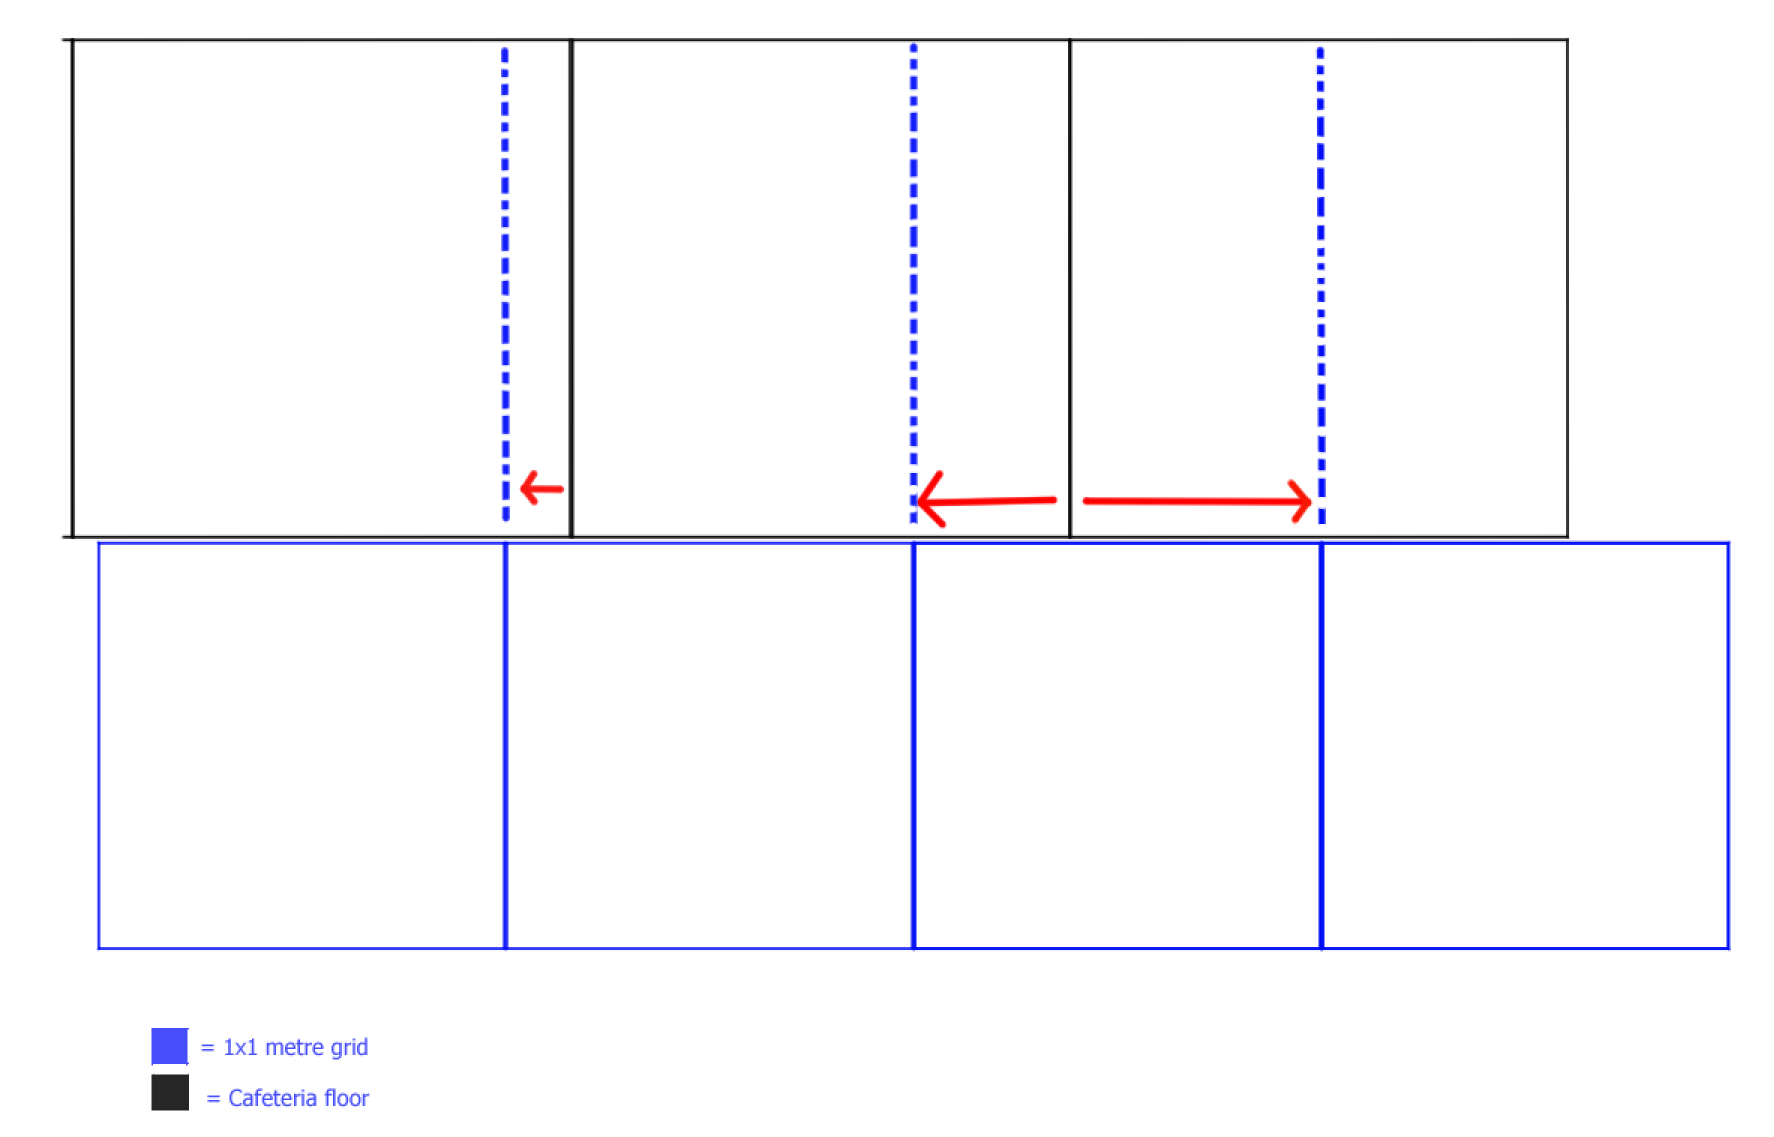
\includegraphics[angle=90, scale=0.22]{meth1.png}}
		\caption{Methodology to divide the cafeteria area into 1x1 metre grids}
		\label{fig1}
	\end{figure}
		\end{comment}
		
	In the cafeteria, the solution was straightforward. We simply measured the difference in distance between the grooves of the standard tiles and those used in the cafeteria. By adjusting the measurements accordingly, we were able to maintain an accurate grid despite the variation in tile type.
	
	\begin{comment}
	\begin{figure}[htbp]
		\centerline{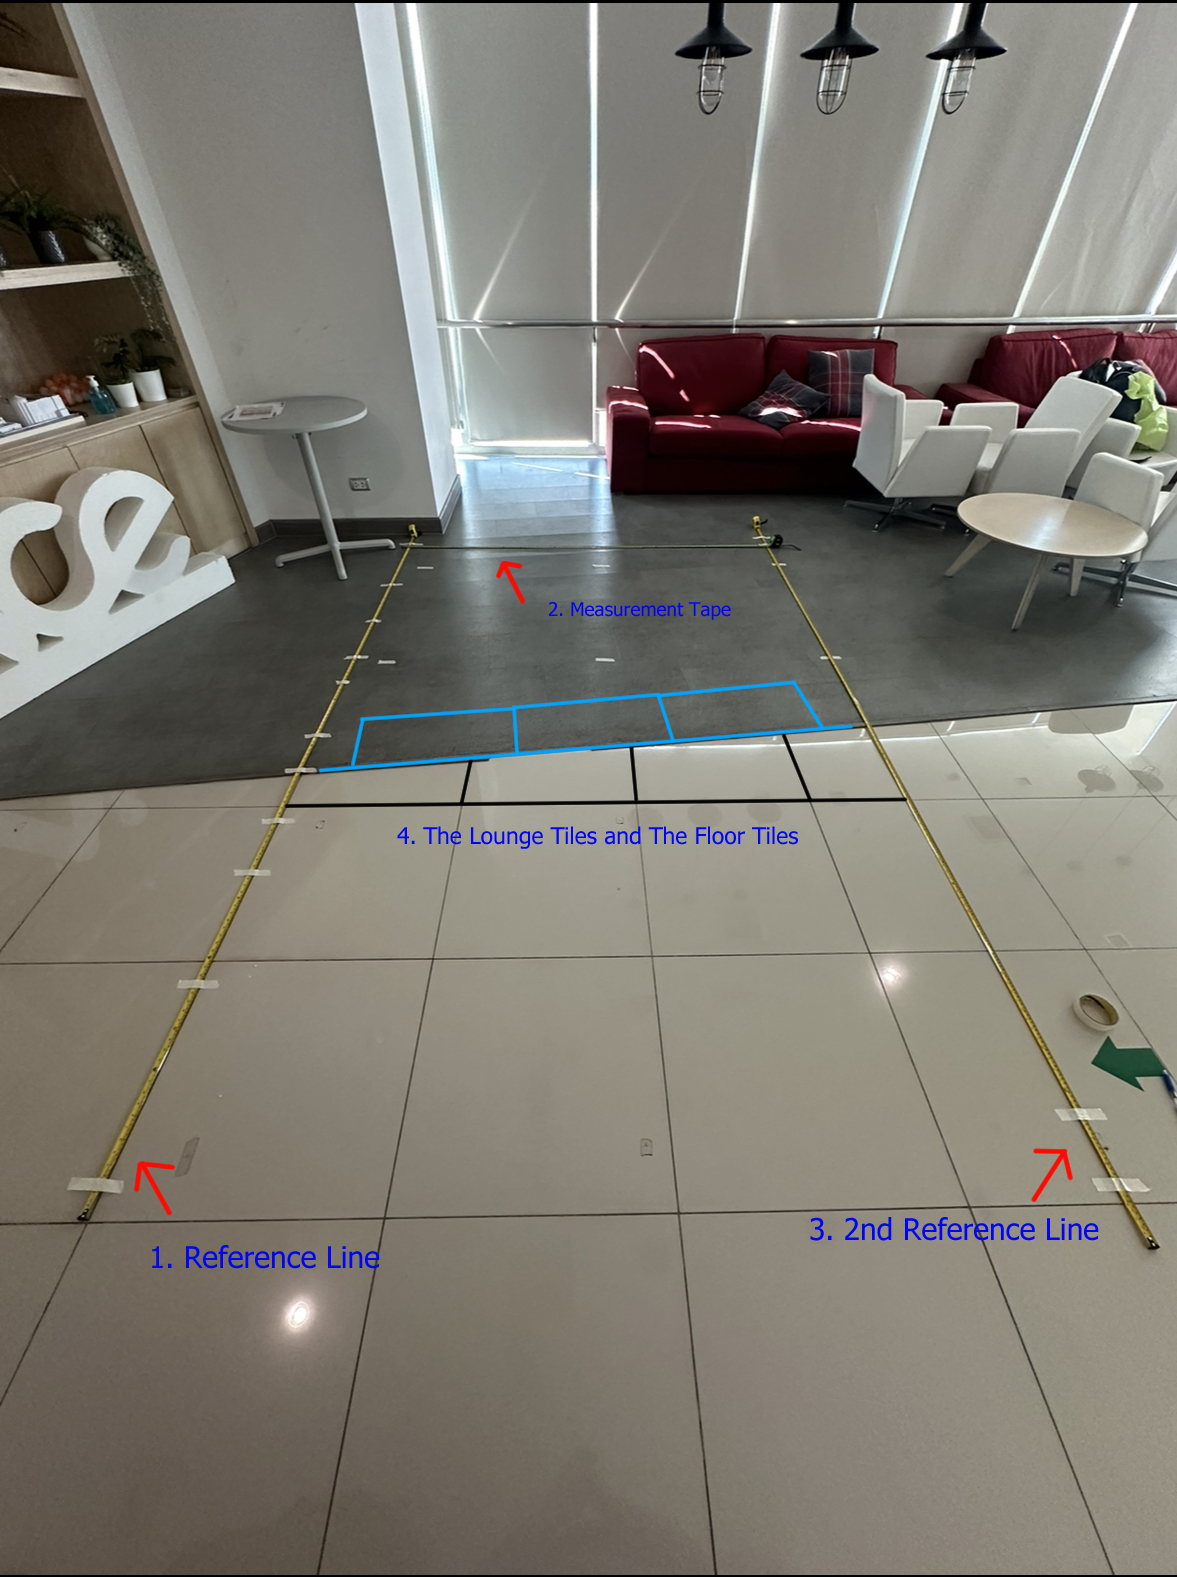
\includegraphics[scale=0.22]{meth2.jpg}}
		\caption{Methodology to divide the lounge area into 1x1 metre grids}
		\label{fig2}
	\end{figure}
	\end{comment}
	
	The lounge area presented a more complex challenge due to the tiles being in different sizes and orientation, as shown by the image above (4.) . To address this, we created a single straight line across the lounge using a tape measure from a fixed point which we proceeded to use as the reference line as shown above. We then took 1-meter measurements using a measuring tape (2.). A second reference line was used to make sure that the measuring tape was straight so that the 1 metre grid would not be slanted.
	Additionally, we had to account for the wear and tear on the area used for our experiment. Human traffic and cleaning activity had the potential to slightly shift or damage the tape, which could impact the grid's accuracy. However, by monitoring and adjusting for any movement in the tape, we were able to maintain the integrity of our measurements throughout the process.
	
	
	The data collected resulted in xxx amount of points collected for floor 7 and xxx amount of points collected for floor 6
	
	
	
	\section{Result}
	The dataset used in this study consisted of 12,640 data points collected across 1x1m\textsuperscript{2} grids distributed among the floors of our experimental setup. By filtering the available BSSID to utilize only SSID with ‘kmitl’ or ‘cmkl’ we end up with 392 unique BSSID, spanning across the 2 floors of the experiment. A rationale behind filtering WiFi signals in this experiment is to determine whether only easily known BSSID can be utilized in implementing IPS. 9019 data points were collected on 6th floor and 3621 data points were collected on 7th floor.
	
	To explore how different parameter settings impact model training, we systematically iterate through various configurations, training the model multiple times under each setting. The table below highlights the best results observed. Notably, the highest accuracy and the best AGT (Adaptive Generalization Tradeoff) do not come from the same parameter setting. This suggests that these metrics prioritize different aspects of performance—optimizing for accuracy does not necessarily yield the best AGT and vice versa. This insight provides a key perspective as we analyze the results in more detail.
	
	\begin{figure}[htbp]
		\centerline{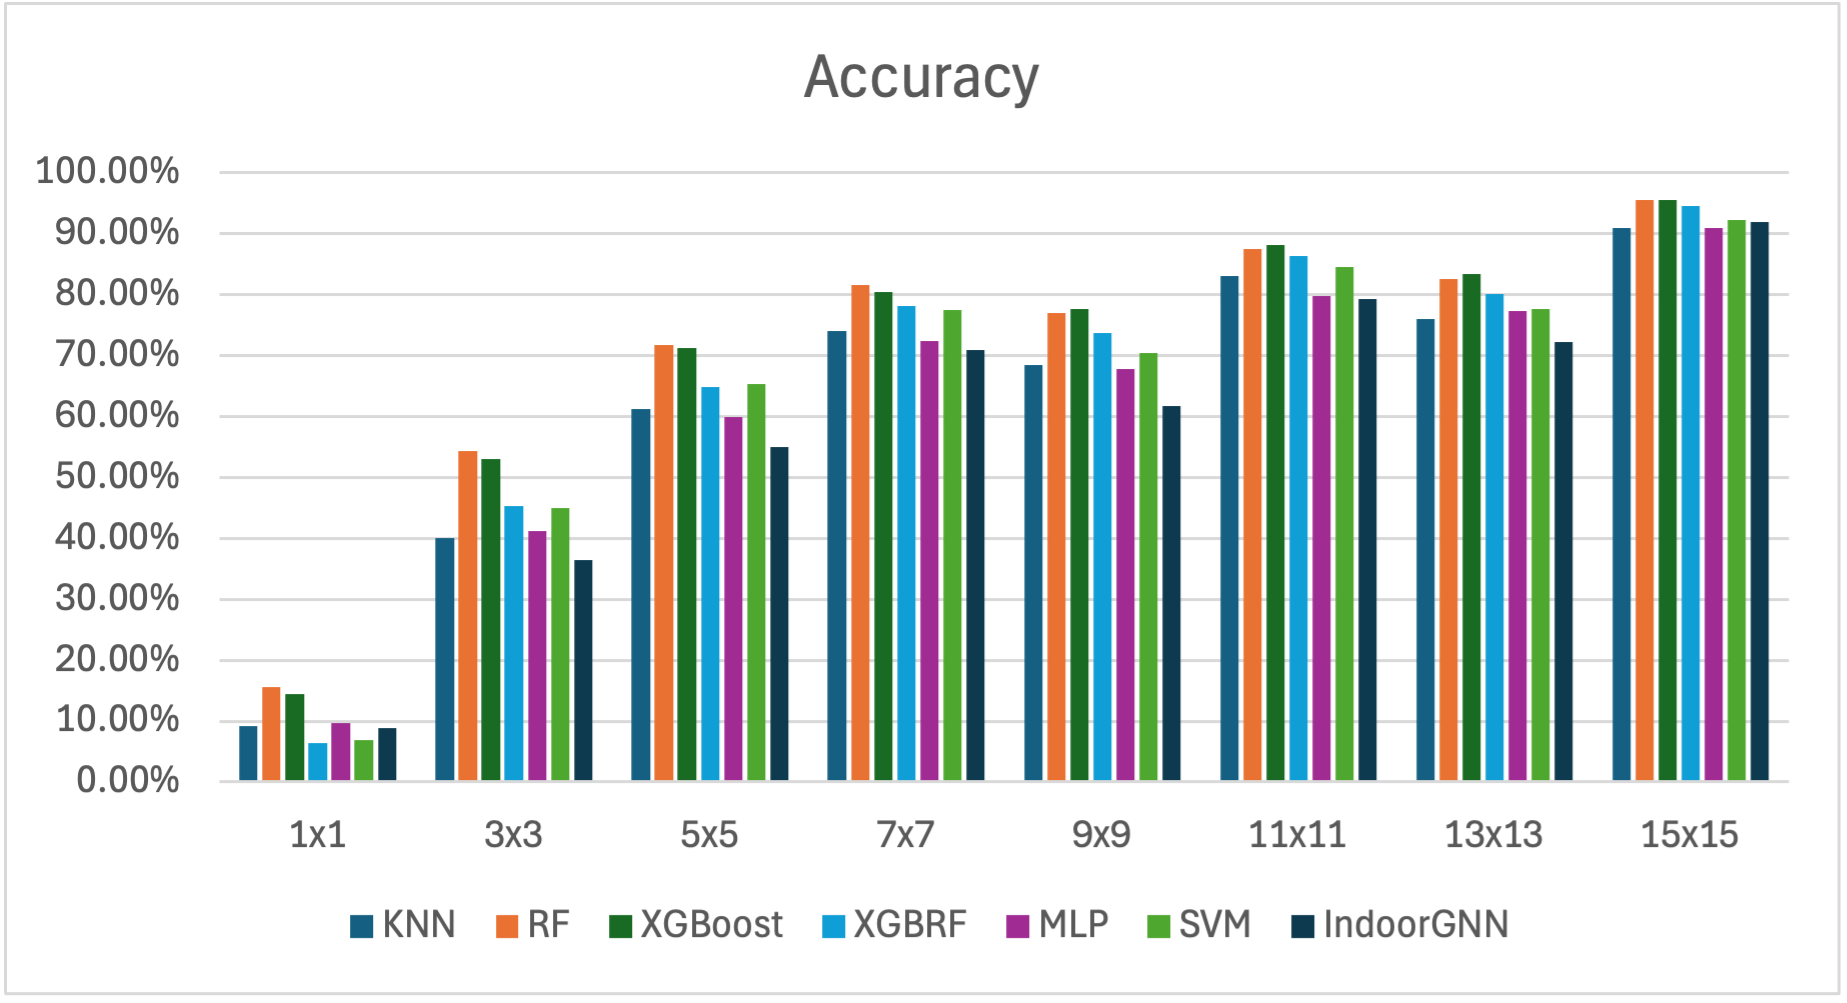
\includegraphics[scale=0.65]{image3.png}}
		\caption{Model Accuracy on Different grid size}
		\label{fig3}
	\end{figure}
	
	\begin{figure}[htbp]
		\centerline{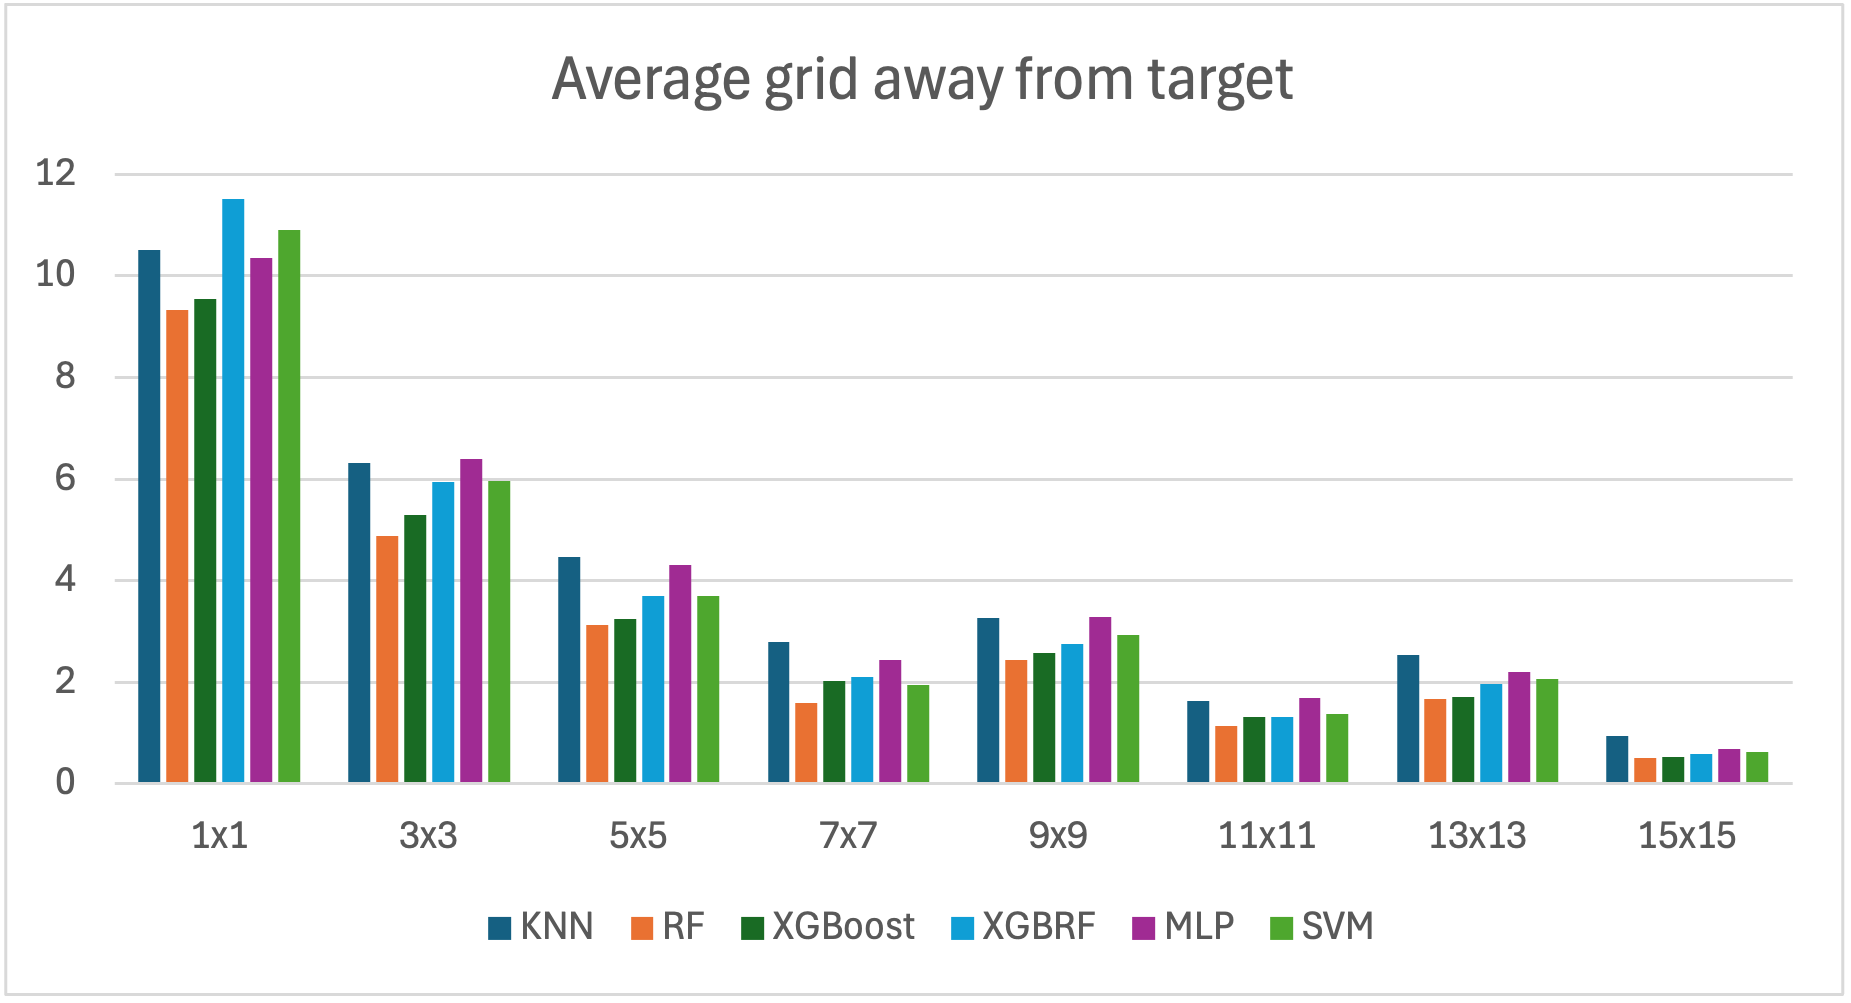
\includegraphics[scale=0.65]{image1.png}}
		\caption{Model Average grid away from Target on Different grid size}
		\label{fig4}
	\end{figure}
	
	To further analyze the spatial distribution of WiFi signals within our test environment, we generated a BSSID heatmap. This visualization helps illustrate how different access points contribute to the overall feature space used in our IPS model. By mapping the signal strength of each detected BSSID across various grid locations, we can better understand signal propagation patterns and identify potential inconsistencies caused by environmental factors such as interference and signal attenuation. The heatmap serves as a diagnostic tool to evaluate the reliability of WiFi-based positioning in our setup. For clarity, readers should ignore the ID and Comment fields in the heatmap, as these are included solely to ensure the data is plotted correctly.
	
	\begin{comment}
	\begin{figure*}[hbt!]
		\centering
		\subfloat[Grid ID 26001008]{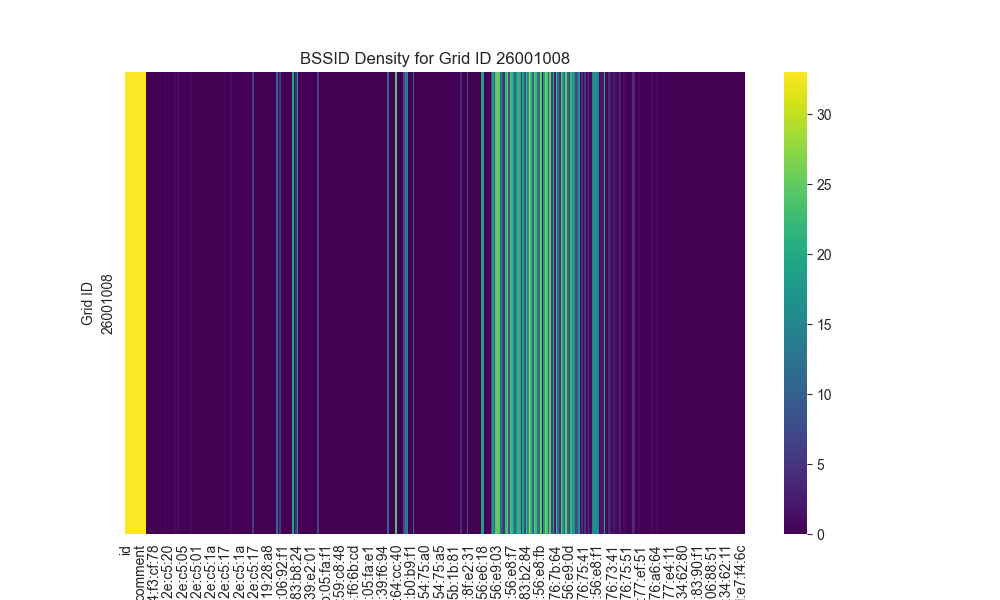
\includegraphics[width=0.45\linewidth]{heatmap_gridid_26001008.png}}
		\subfloat[Grid ID 270011123]{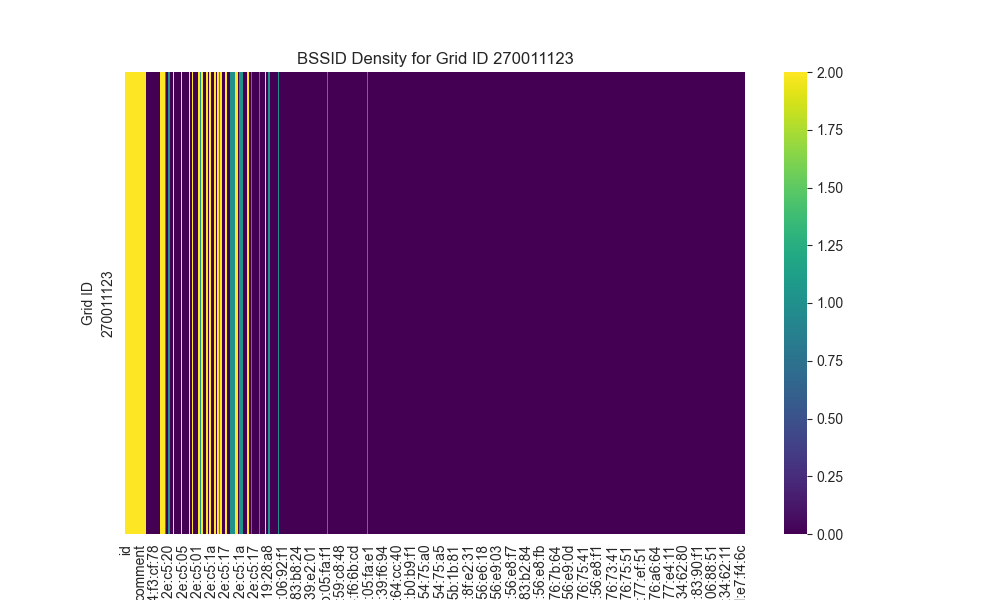
\includegraphics[width=0.45\linewidth]{heatmap_gridid_270011123.png}} \\
		
		\subfloat[Grid ID 26001407]{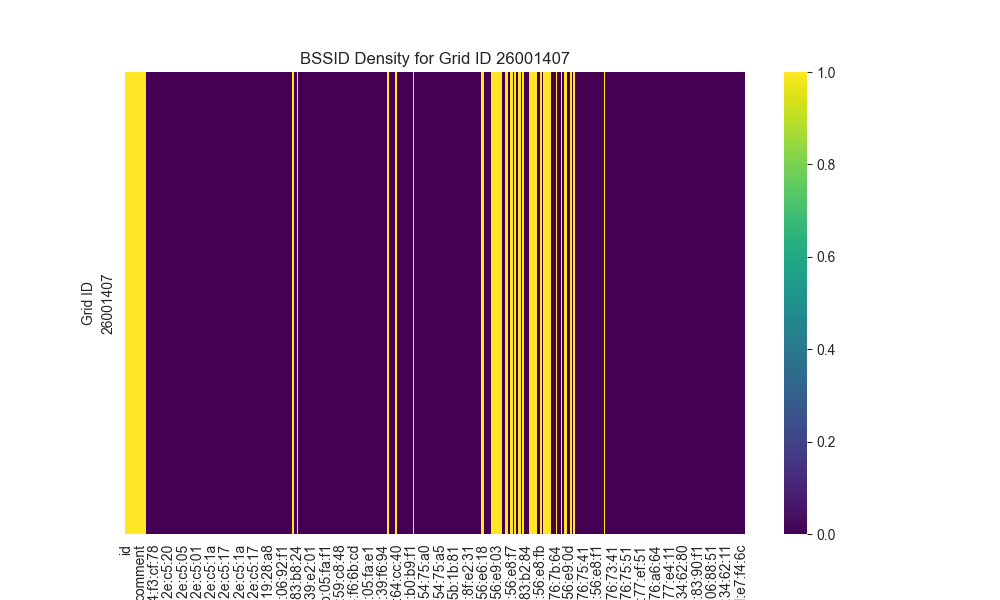
\includegraphics[width=0.45\linewidth]{heatmap_gridid_26001407.png}}
		\subfloat[Grid ID 27001786]{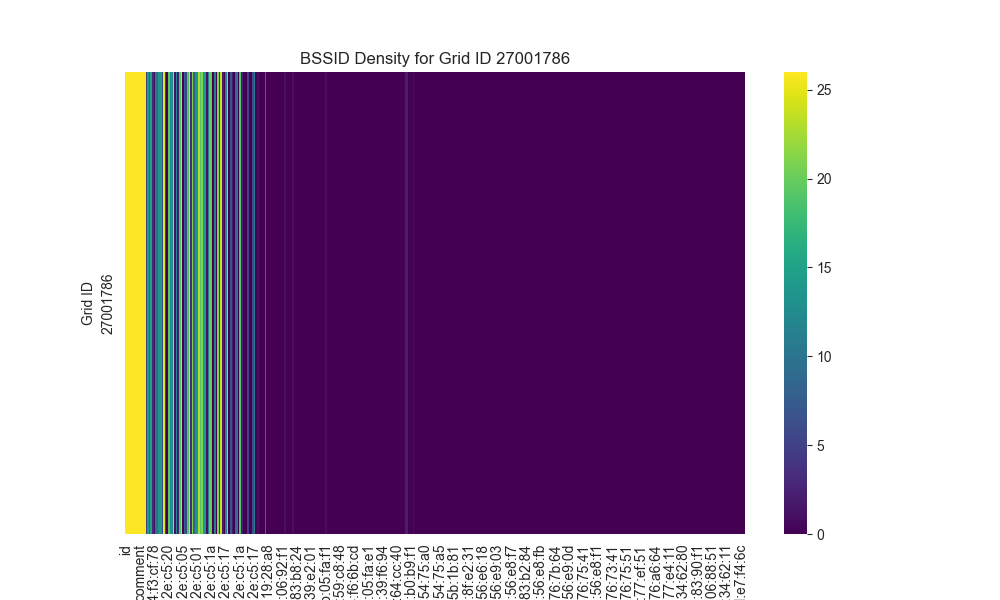
\includegraphics[width=0.45\linewidth]{heatmap_gridid_27001786.png}} \\
		
		\subfloat[Grid ID 26001811]{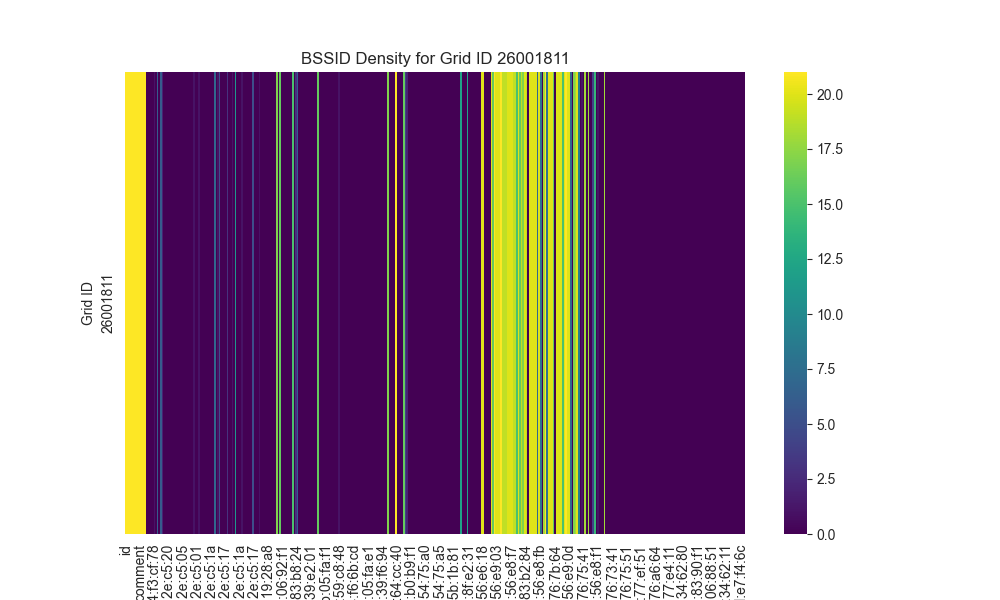
\includegraphics[width=0.45\linewidth]{heatmap_gridid_26001811.png}}
		\subfloat[Grid ID 27001918]{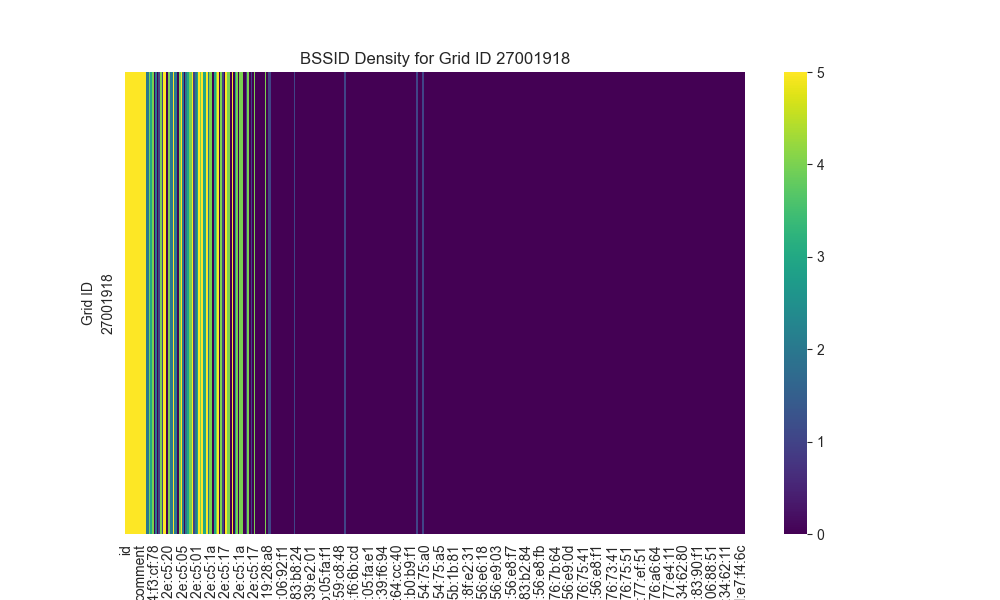
\includegraphics[width=0.45\linewidth]{heatmap_gridid_27001918.png}} \\
		
		\subfloat[Grid ID 26001888]{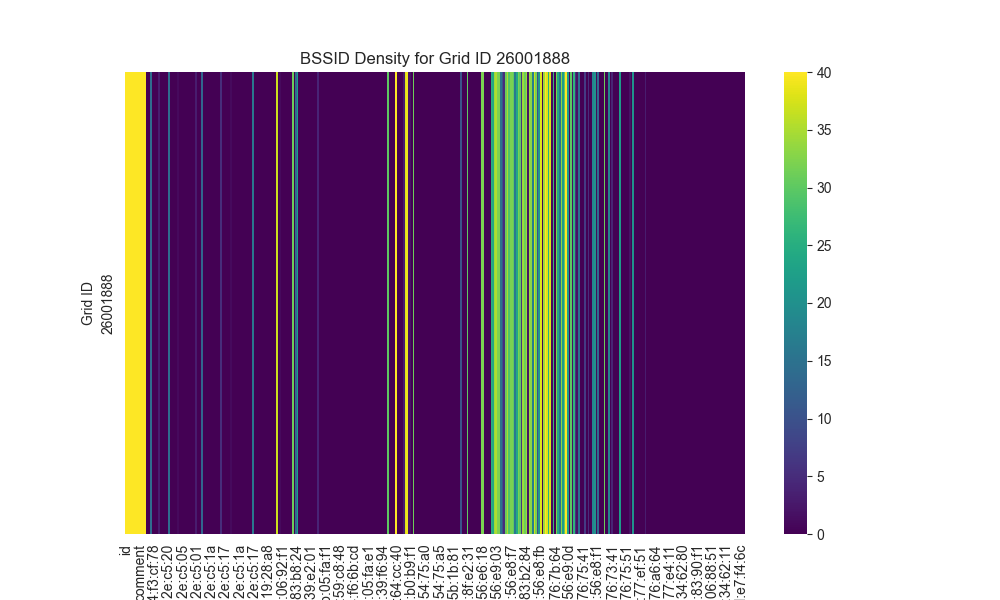
\includegraphics[width=0.45\linewidth]{heatmap_gridid_26001888.png}}
		\subfloat[Grid ID 270011051]{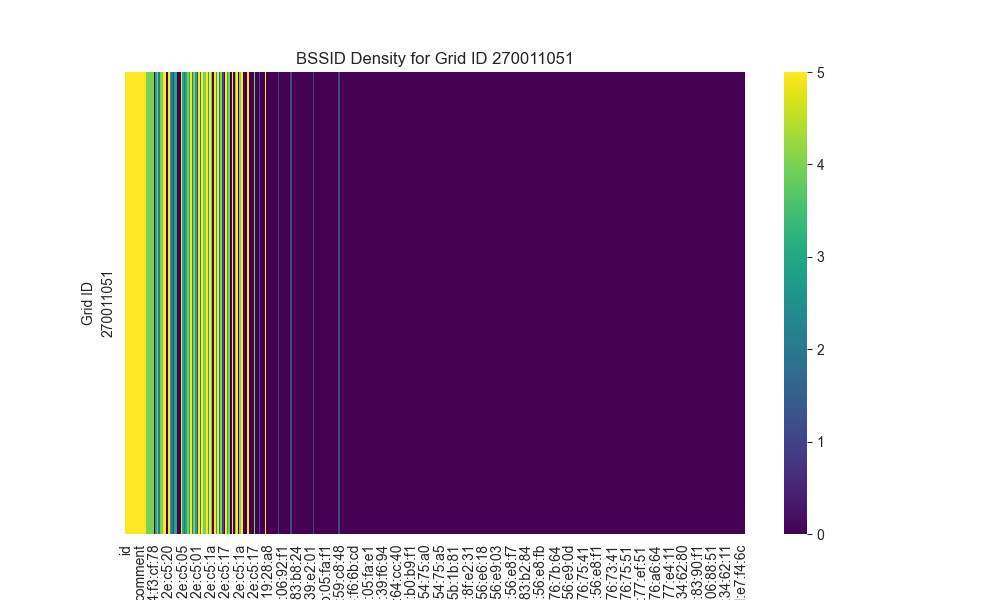
\includegraphics[width=0.45\linewidth]{heatmap_gridid_270011051.png}} \\
		
		\subfloat[Grid ID 260011369]{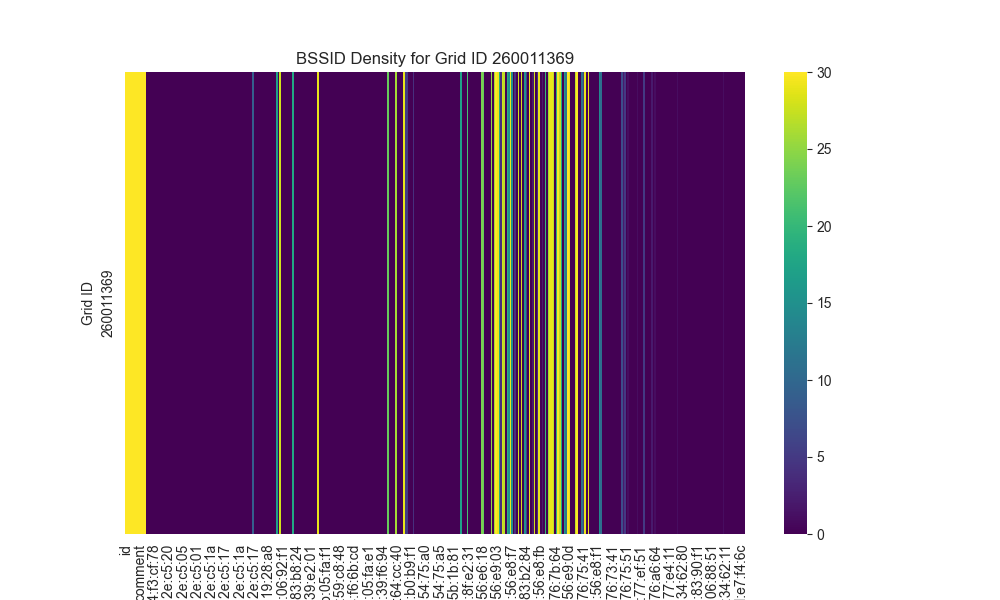
\includegraphics[width=0.45\linewidth]{heatmap_gridid_260011369.png}}
		\subfloat[Grid ID 270011105]{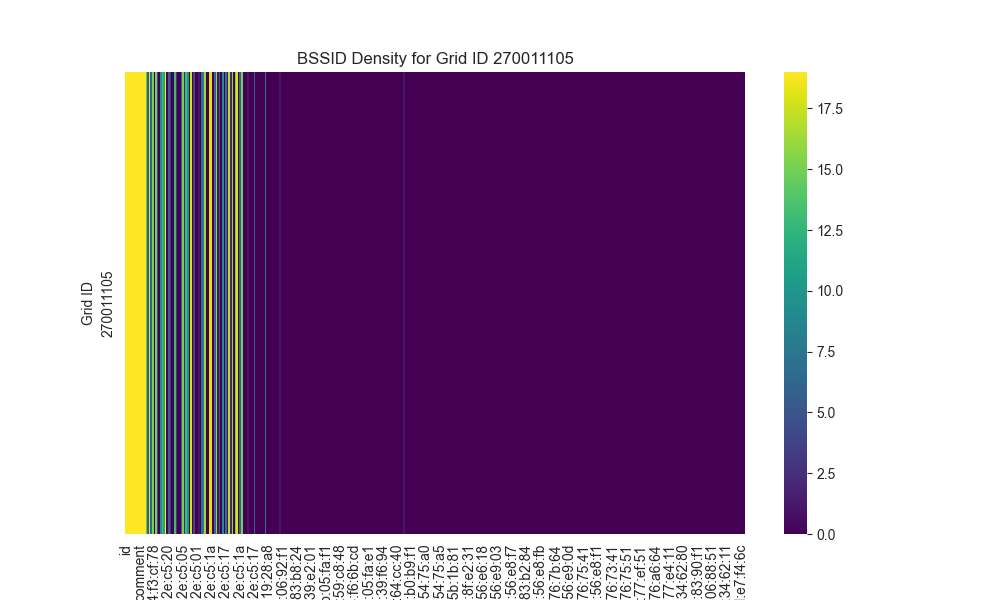
\includegraphics[width=0.45\linewidth]{heatmap_gridid_270011105.png}}
		
		\caption{BSSID Density Heatmaps for Grid IDs (26XXXX on the left, 27XXXX on the right).}
		\label{fig:gay}
	\end{figure*}
	\end{comment}
	
	
	\section{Discussion}
	By conducting our experiment across multiple grid sizes, we can visualize the tradeoff between grid size and precision. To quantify this, we calculate the average grid deviation from the target and multiply it by each grid size’s diagonal length, as shown in (insert fig number). This figure illustrates the expected deviation in predictions when a model is trained on a specific grid size, should an error occur.
	
	While a 15×15m grid size performs well on the graph, it inherently limits accuracy to that resolution. In cases where predictions are correct, the location remains constrained within a 15×15m area, which may not be suitable for applications requiring higher precision—such as those needing to pinpoint areas smaller than this grid size.
	
	Through this experiment, we find that a 7×7m grid size offers the best balance between accuracy and precision. It minimizes error while remaining small enough for use in precision-dependent applications. However, it is important to note that these findings may not generalize to all IPS implementations in different environments. The results suggest that increasing grid size does not necessarily improve accuracy; in some cases, performance actually declines, as shown in the chart. This highlights the need for careful consideration when selecting a grid size based on the specific requirements of an IPS deployment.
	
	\begin{figure}[htbp]
		\centerline{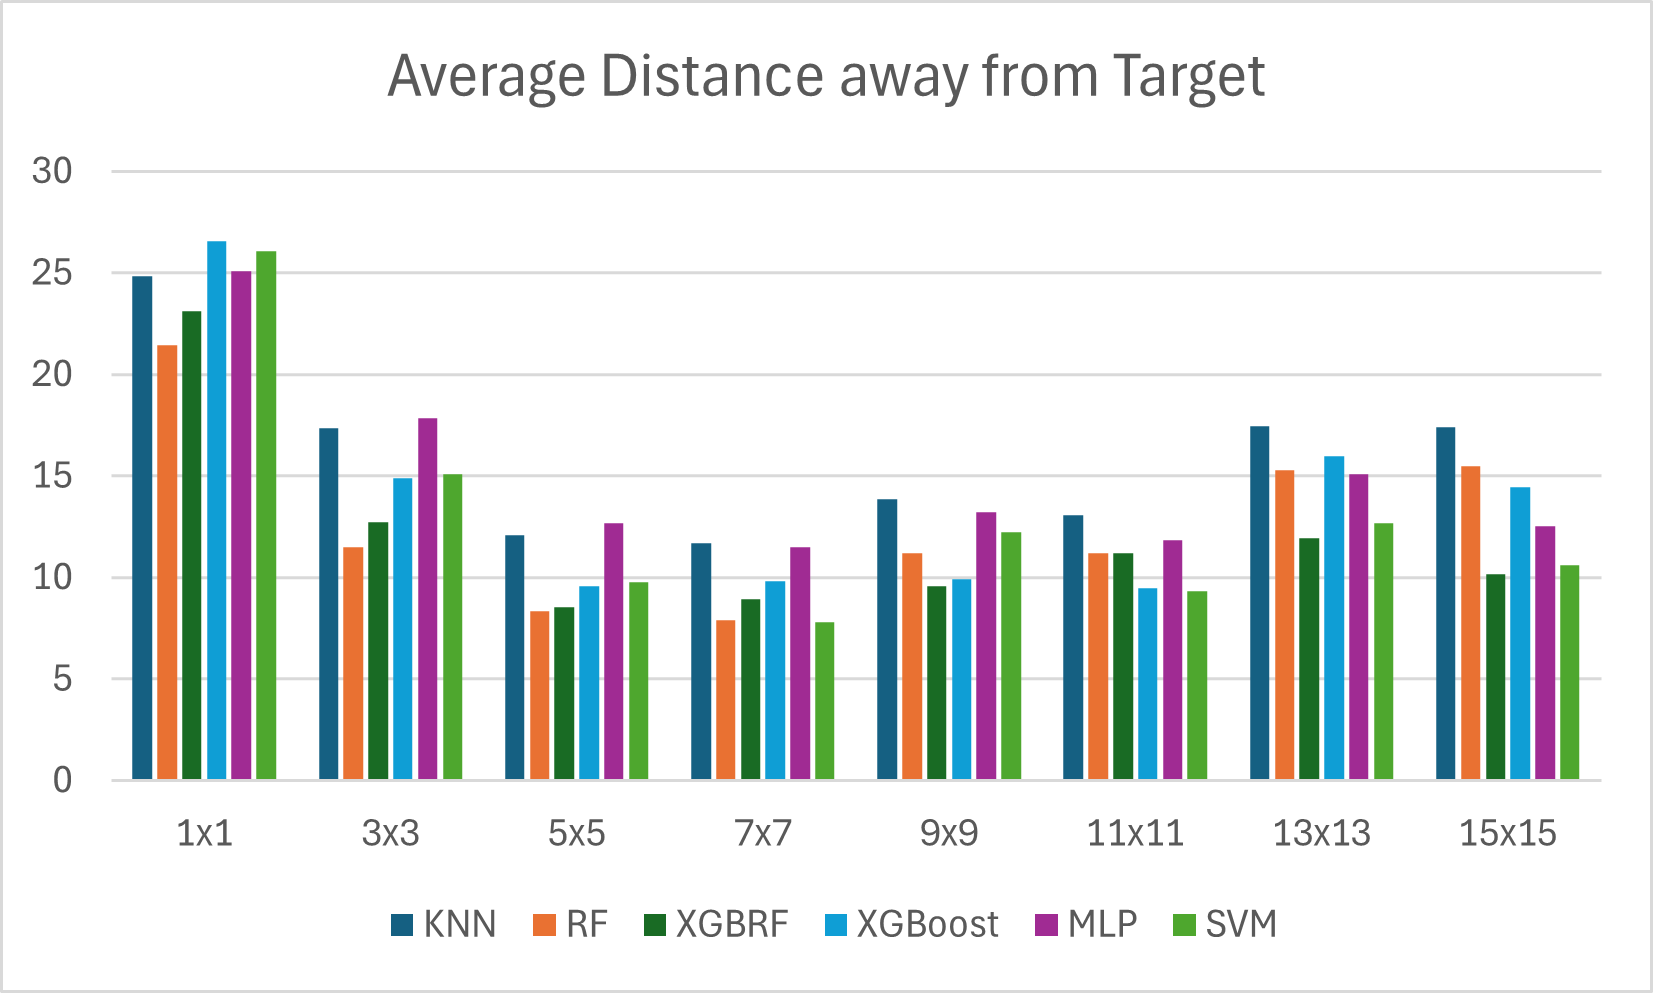
\includegraphics[scale=0.65]{image2.png}}
		\caption{Average Distance Error Across Different Grid Resolutions}
		\label{fig5}
	\end{figure}
	
	Training an IPS model involves significant computational challenges, particularly when dealing with high-dimensional feature spaces. In our experiment, we implemented a simple Wi-Fi access point filtering approach, selecting only access points containing cmkl and kmitl in their names. This drastically reduced the number of access points used as features, making the training process more efficient.
	
	With this filtering method, we were able to train models across multiple grid sizes (1×1, 3×3, 5×5, 7×7, 9×9, 11×11, 13×13, and 15×15) within four days. In contrast, the unfiltered dataset took six days to complete training for just the 1×1 grid size across all target models we intended to test. Due to computational constraints—specifically, the complexity exceeding the capabilities of a single RTX 3080 Ti—we were unable to conduct further experiments with the unfiltered dataset.
	
	Interestingly, our results indicate that filtering access points did not negatively impact the model's learning process. A comparison of training trajectories for the 1×1 grid experiment shows that the filtered model performed comparably to the unfiltered one, if not slightly better in terms of convergence. This suggests that reducing feature dimensionality not only accelerates training but may also make learning more stable.
	
	\begin{figure*}[hbt!]
		\centering
		\begin{minipage}{0.45\textwidth}
			\centering
			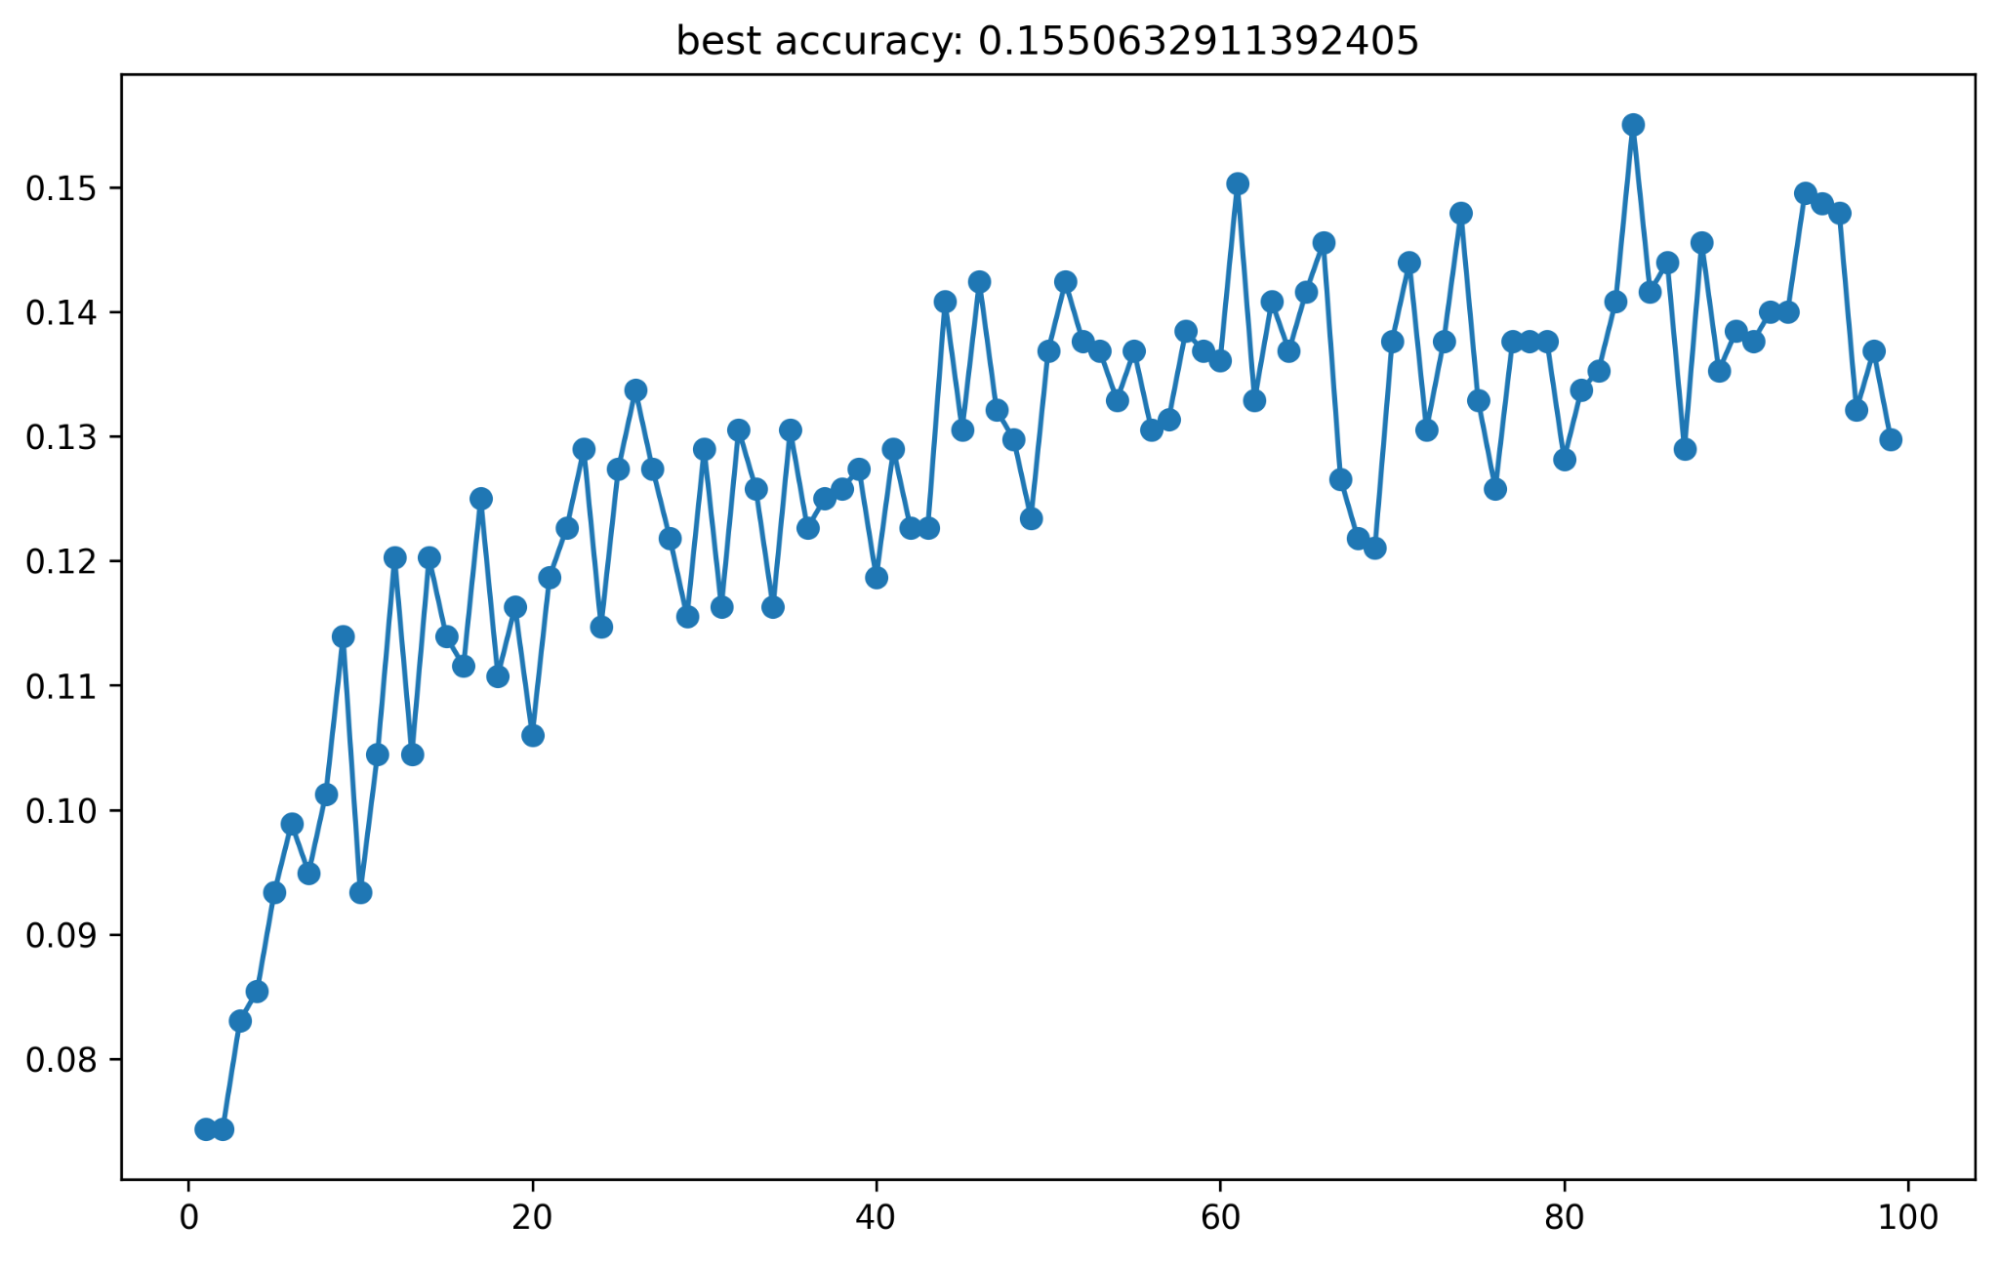
\includegraphics[width=\linewidth]{image5.png}
			\caption{RF Model accuracy with BSSID filtering (1x1)} % Caption without numbering
			
			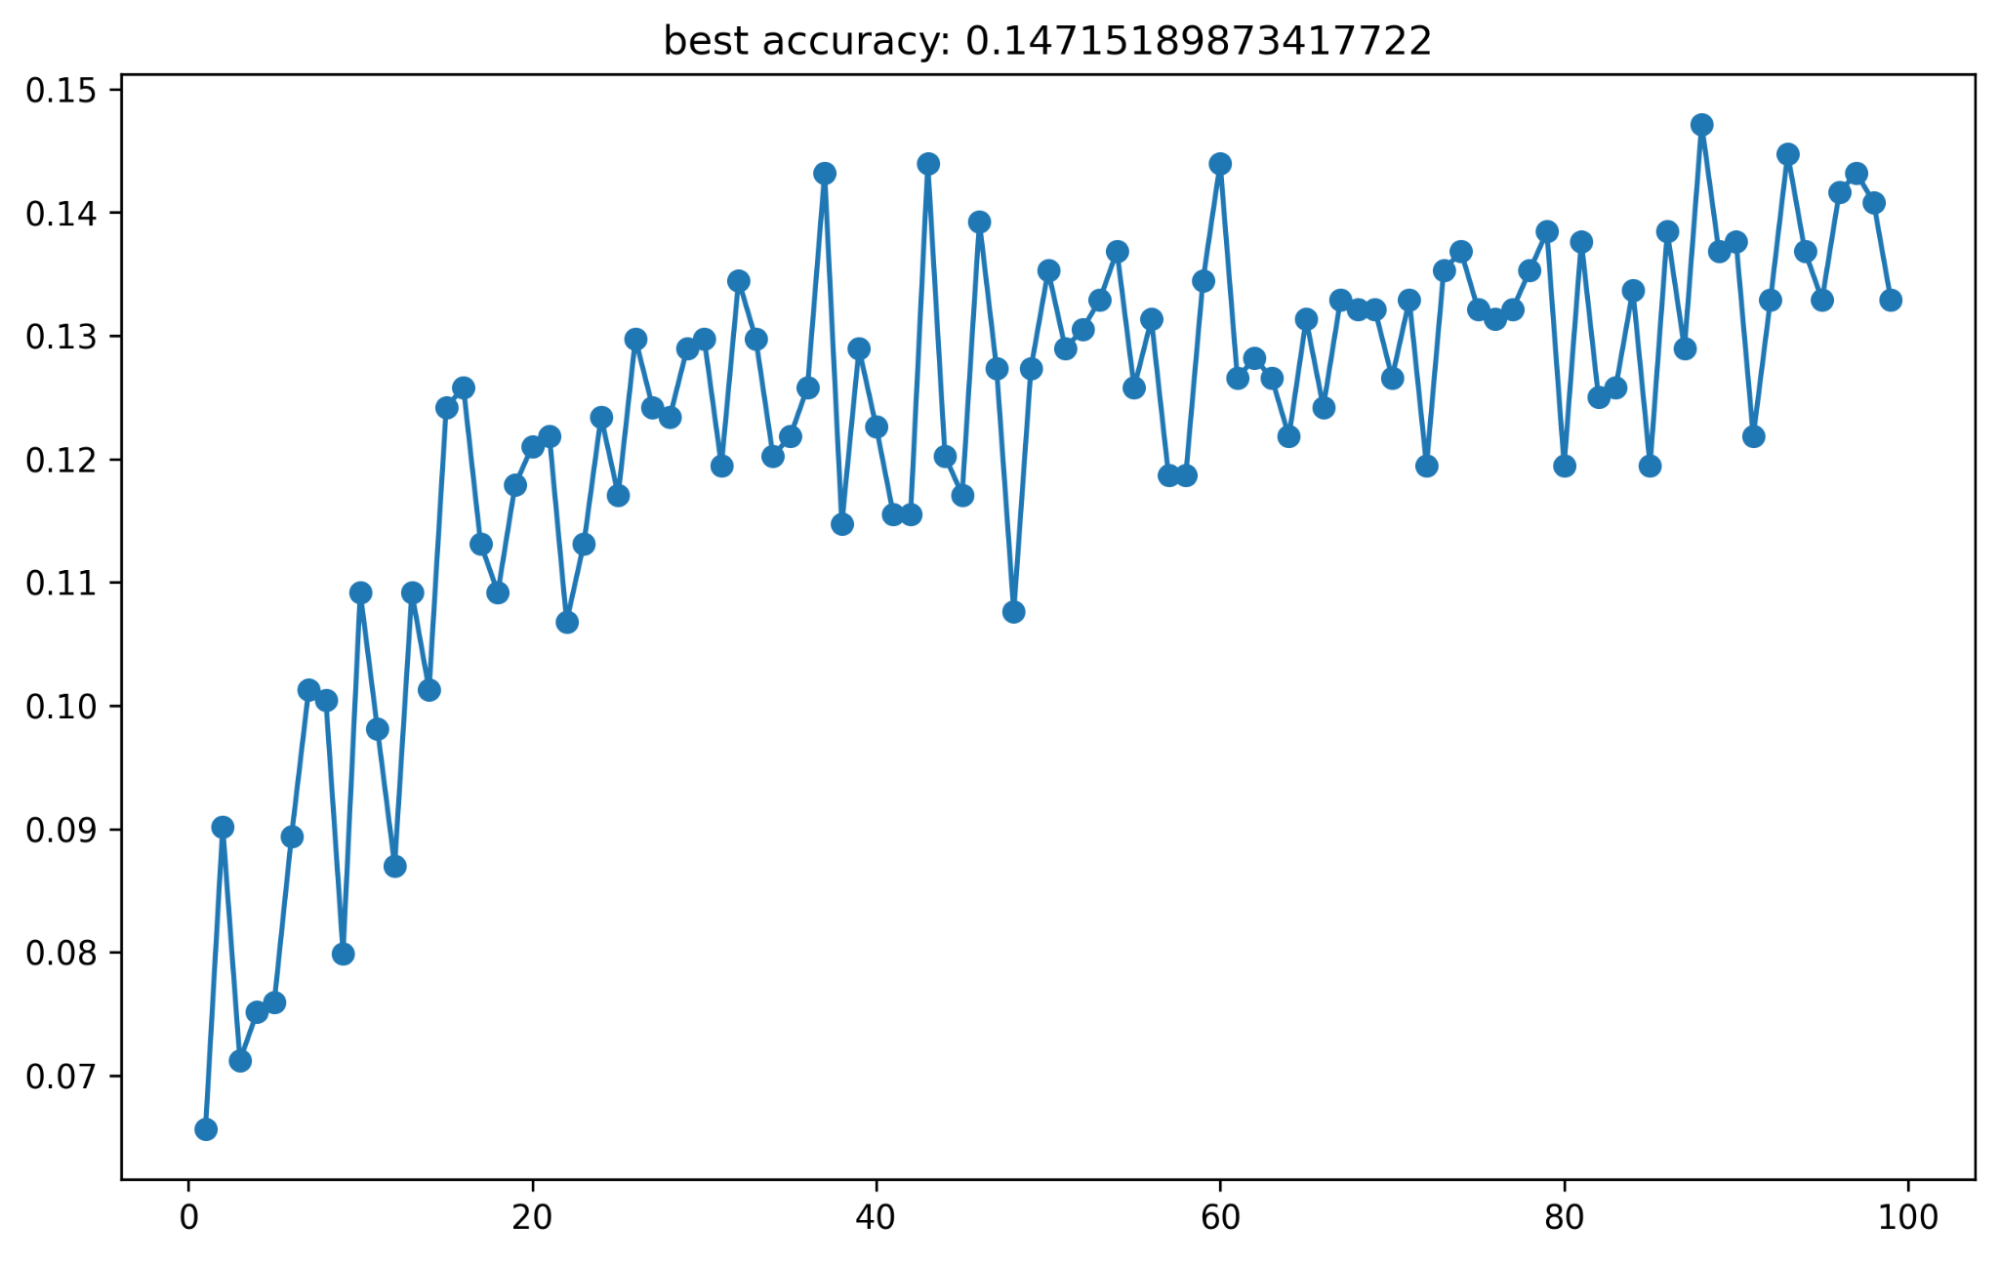
\includegraphics[width=\linewidth]{image6.png}
			\caption{RF Model AGT with BSSID filtering(1x1)}
		\end{minipage}
		\hfill
		\begin{minipage}{0.45\textwidth}
			\centering
			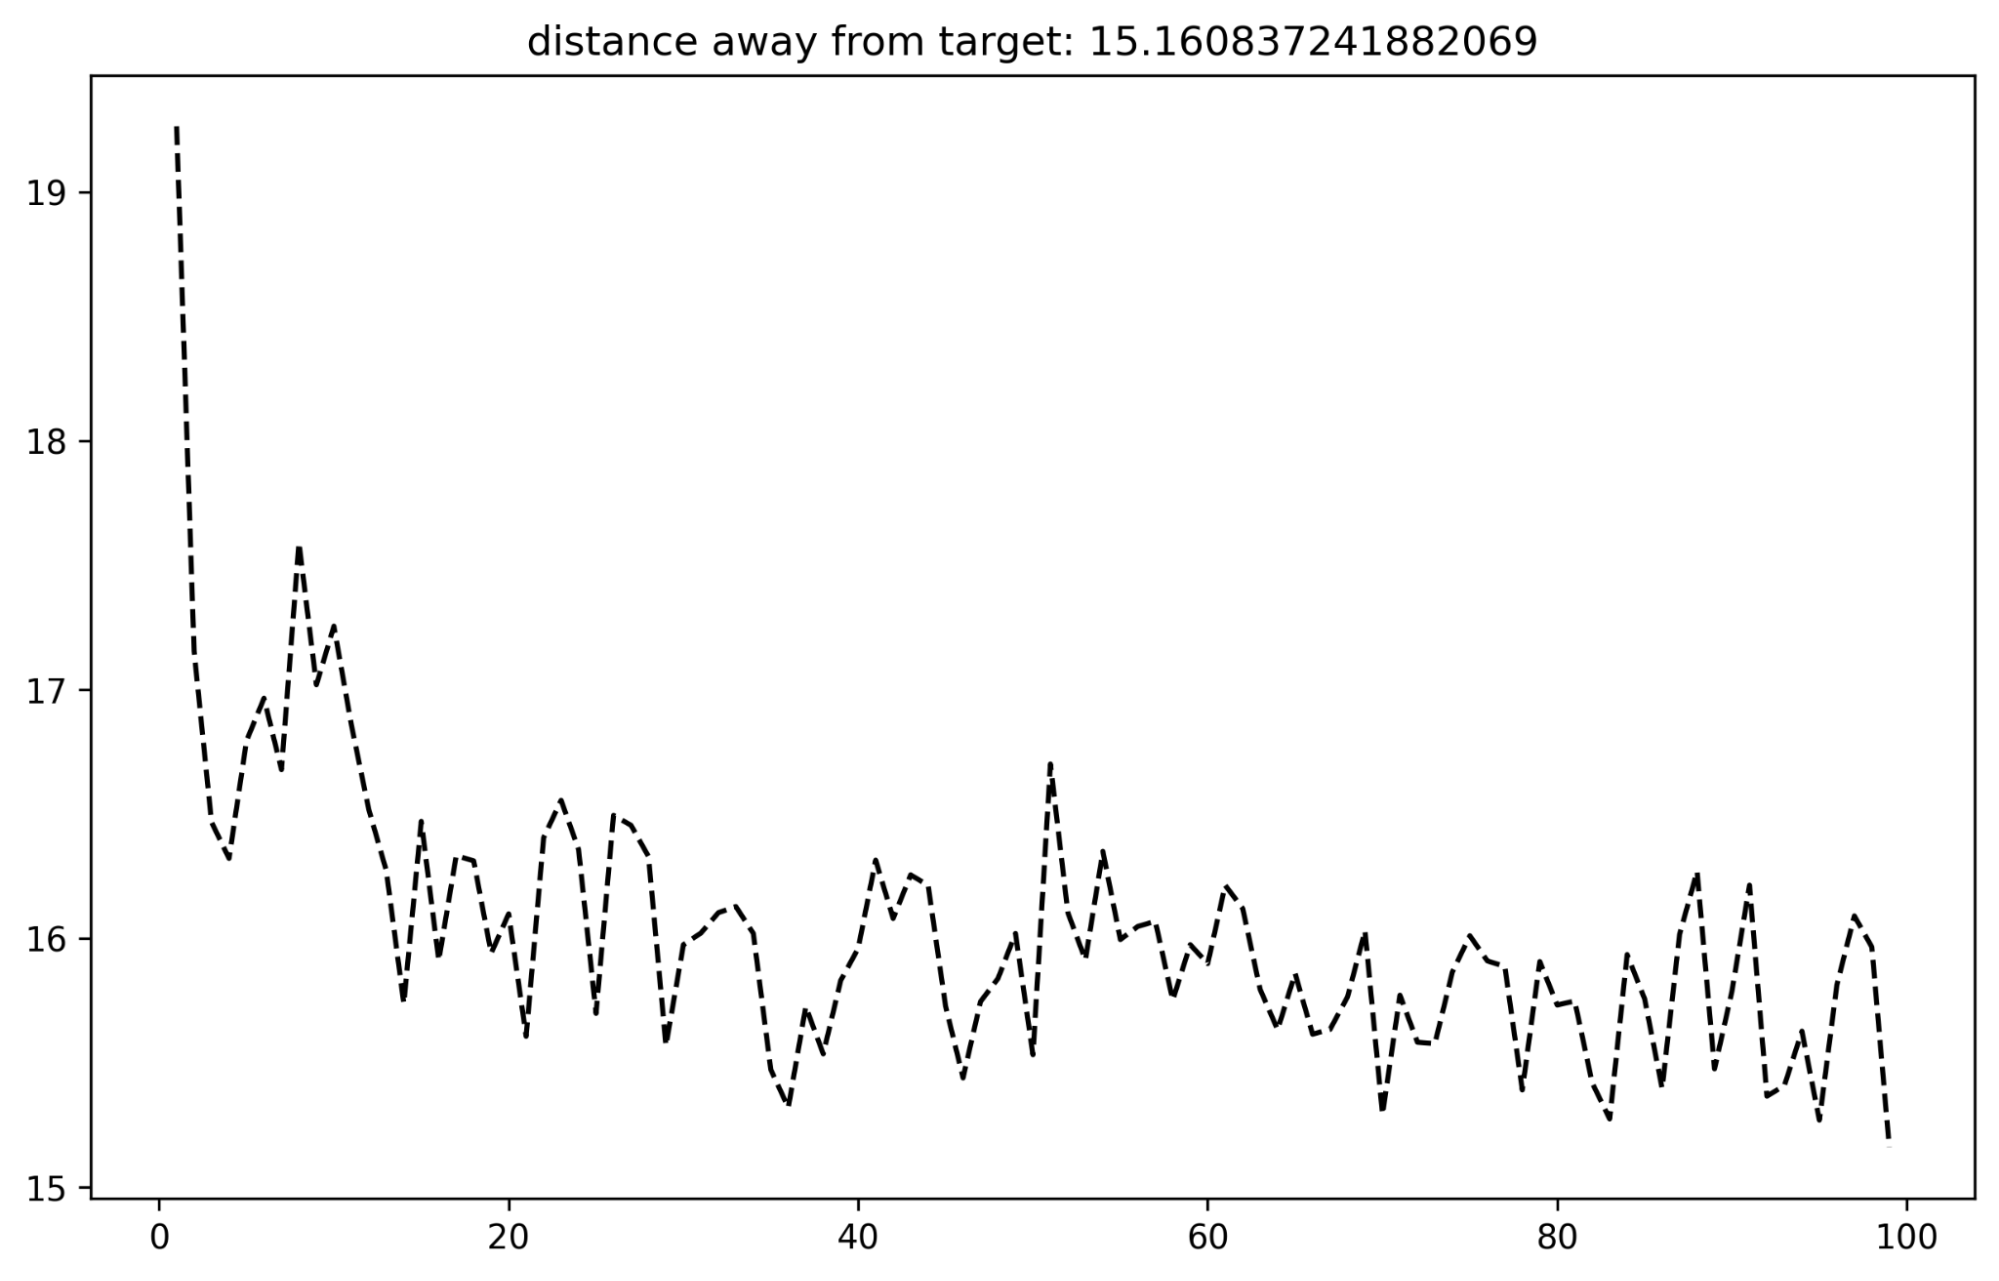
\includegraphics[width=\linewidth]{image4.png}
			\caption{RF Model accuracy without BSSID filtering(1x1)}
			
			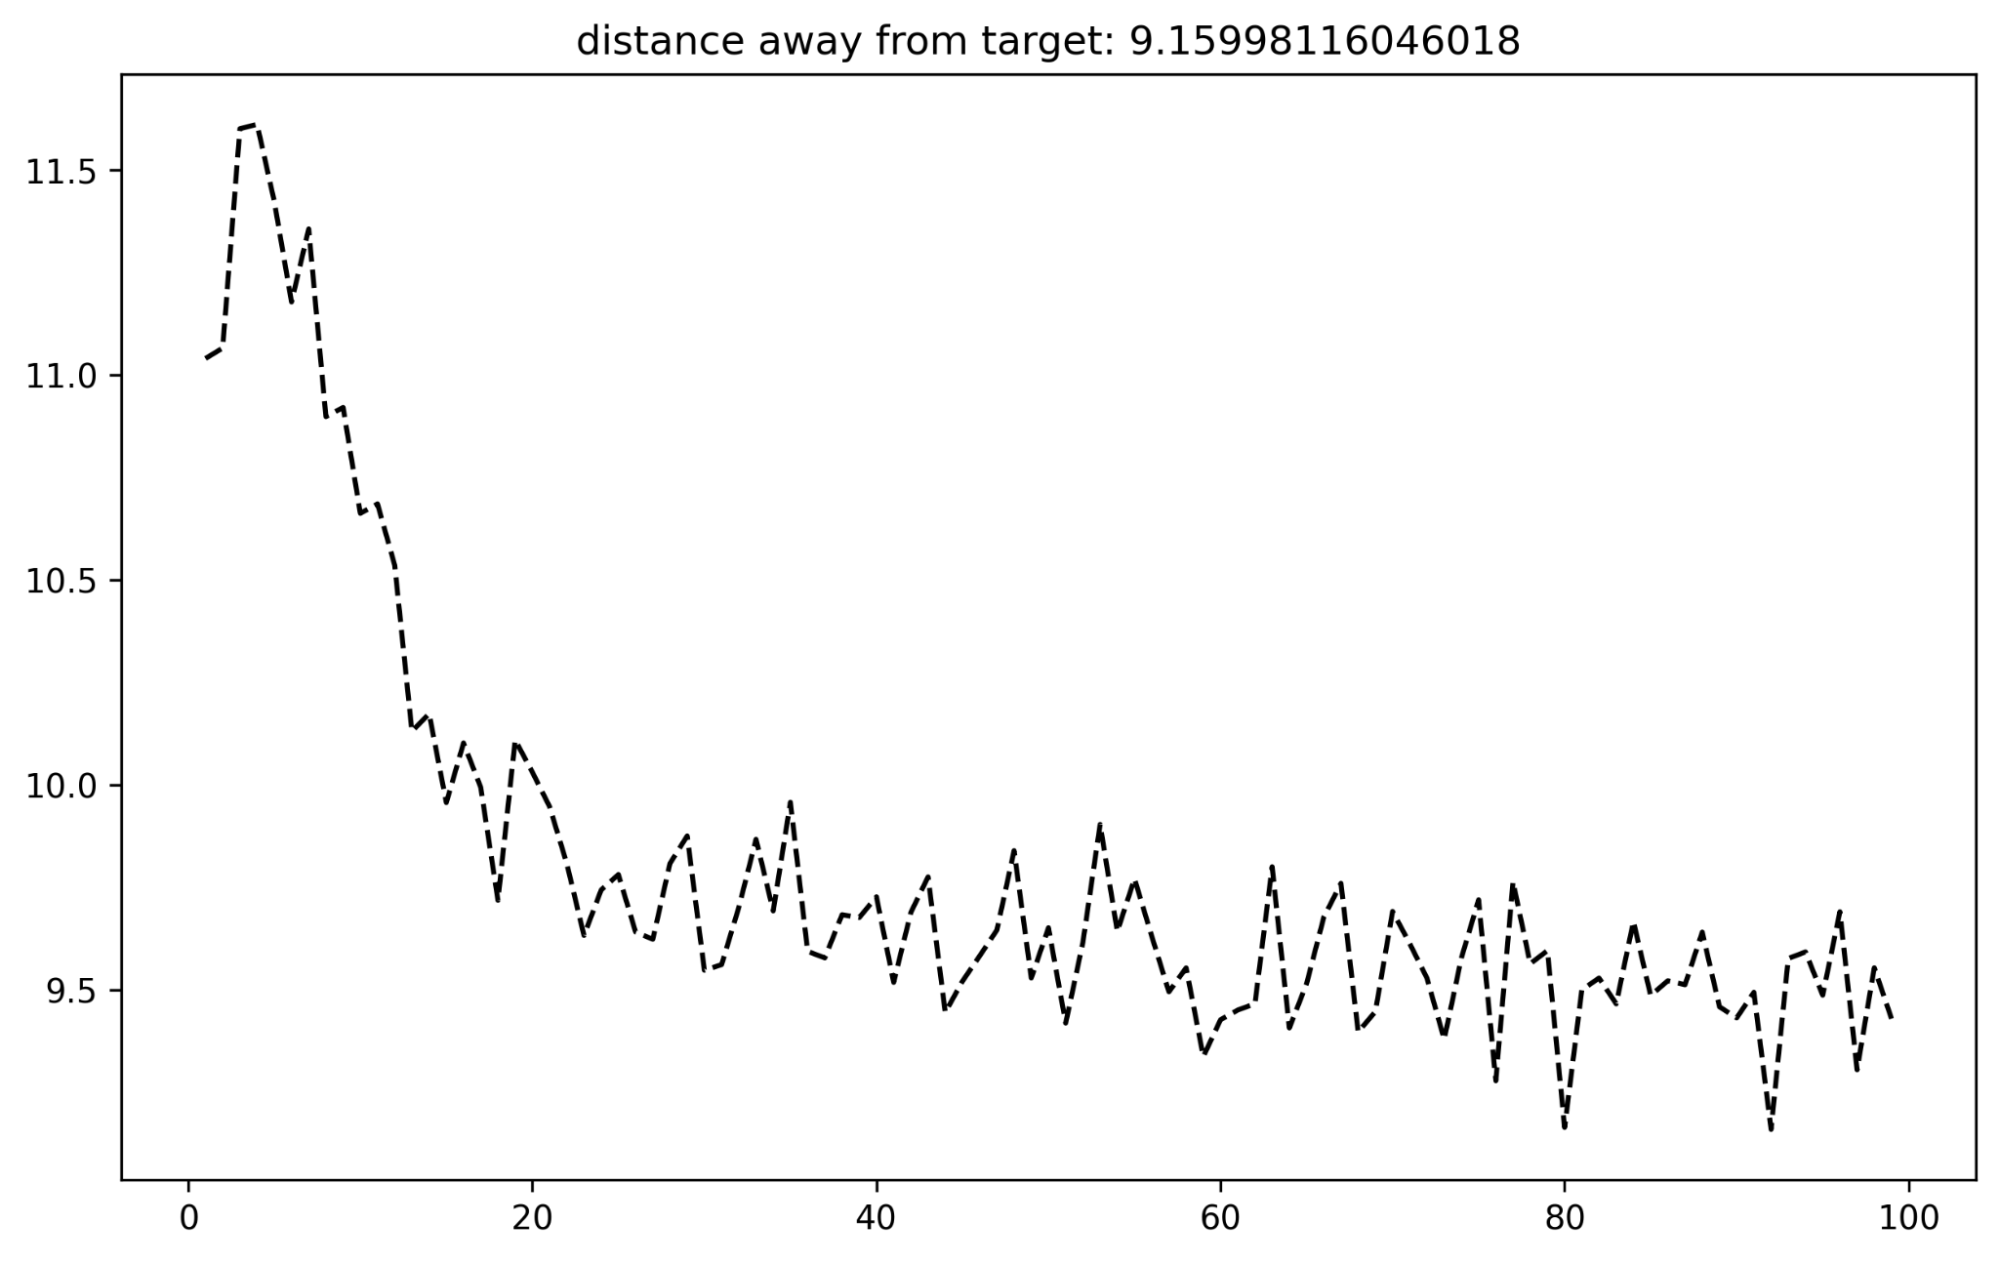
\includegraphics[width=\linewidth]{image7.png}
			\caption{RF Model AGT without BSSID filtering(1x1)}
		\end{minipage}
	\end{figure*}
	
	
	
	\section{Conclusion}
	In conclusion, this paper extends our previous work by refining the implementation of an IPS using a classification-based approach. Through our experiments across multiple grid sizes, we visualized the trade-offs between grid size and precision, showing that increasing grid size does not necessarily improve accuracy and may, in some cases, lead to worse performance. Our findings suggest that a 7×7m grid size offers the best balance between accuracy and precision, making it suitable for applications that require finer localization. However, we acknowledge that these results may not generalize to all environments due to variations in WiFi signal behavior and building structures.
	
	Additionally, we implemented a simple filtering method to limit the number of WiFi BSSID features, preventing excessive model complexity while maintaining comparable performance to an unfiltered approach. This method significantly reduced training time and computational requirements, allowing us to complete model training across multiple grid sizes efficiently. Our results indicate that reducing feature dimensionality not only accelerates training but may also contribute to more stable learning. To better assess IPS performance, we introduced two new evaluation metrics—Average Grid from Target (AGT) and Average Distance from Target (ADT)—which provide a clearer understanding of prediction deviation. Ultimately, our study highlights key considerations in IPS design, particularly in grid size selection and feature filtering, and offers insights for improving indoor positioning accuracy in practical implementations.
	
	\begin{thebibliography}{00}
		\bibitem{bgp1} A, Nessa, B. Adhikari, F. Hussain and X. N. Fernando, A Survey of Machine Learning for Indoor Positioning," in IEEE Access, vol. 8, pp. 214945-214965, 2020, doi: 10.1109/ACCESS.2020.3039271
		\bibitem{bgp2} H. A. de Souza Mourão and H. A. B. F. de Oliveira, Indoor Localization System Using Fingerprinting and Novelty Detection for Evaluation of Confidence in Future Internet ,14(2) , 51. 2022, doi:  https://doi.org/10.3390/fi14020051 
		\bibitem{bgp3} H.T. Gidey, X. Guo, K. Zhong, L. Li, Y. Zhang. OHetTLAL: An Online Transfer Learning Method for Fingerprint-Based Indoor Positioning in  Sensors 2022, 22(23), 9044, doi: https://doi.org/10.3390/s22239044
		\bibitem{bgp4} H. Obeidat, W. Shuaieb, O. Obeidat, and R. Abd-Alhameed, "A Review of Indoor Localization Techniques and Wireless Technologies," *Wireless Personal Communications*, vol. 119, no. 1, pp. 289–327, Jul. 2021, doi: 10.1007/s11277-021-08209-5.
		\bibitem{bg2} D. Csik, Á. Odry, and P. Sarcevic, "Comparison of RSSI-Based Fingerprinting Methods for Indoor Localization," in *Proc. 20th IEEE International Symposium on Intelligent Systems and Informatics (SISY)*, Subotica, Serbia, Sep. 2022, pp. 000273–000278, doi: 10.1109/SISY56759.2022.10036270.
		\bibitem{LRE1} B. Intachuen, M. Charoenphon, T. Mankhetwit (2024), Classification-based-IPS [Online]. Available: \url{https://github.com/RinRin-32/Classification-based-IPS}
		\bibitem{LRE2} R. Vishwakarma, R. B. Joshi, and S. Mishra. IndoorGNN: A Graph Neural Network based approach for Indoor Localization using WiFi RSSI, In Big Data and Artificial Intelligence: 11th International Conference, BDA 2023, 150–165, \url{doi:https://doi.org/10.1007/978-3-031-49601-1_11}
		\bibitem{LRE3} D. Christodoulou,  Developing an indoor localisation and wayfinding app for a University Library Available: \url{https://project-archive.inf.ed.ac.uk/ug4/20223034/ug4_proj.pdf}
		\bibitem{LRE4} L. Bibbo, R. Carotenuto, F. D. Corte, An Overview of Indoor Localization System for Human Activity Recognition (HAR) in Healthcare in Sensors 22, no. 21: 8119, doi: \url{https://doi.org/10.3390/s22218119}
		\bibitem{LRE5}N. A. Maung Maung, B. Y. Lwi and S. Thida, "An Enhanced RSS Fingerprinting-based Wireless Indoor Positioning using Random Forest Classifier," 2020 International Conference on Advanced Information Technologies (ICAIT), Yangon, Myanmar, 2020, pp. 59-63, doi: 10.1109/ICAIT51105.2020.9261776.
		
	\end{thebibliography}
	\vspace{12pt}
	\color{red}
	IEEE conference templates contain guidance text for composing and formatting conference papers. Please ensure that all template text is removed from your conference paper prior to submission to the conference. Failure to remove the template text from your paper may result in your paper not being published.
	
	
	\clearpage
	\begin{comment}
	\begin{figure*}[hbt!]
		\centering
		% Left Column (26XXXX IDs)
		\begin{minipage}{0.45\textwidth}
			\centering
			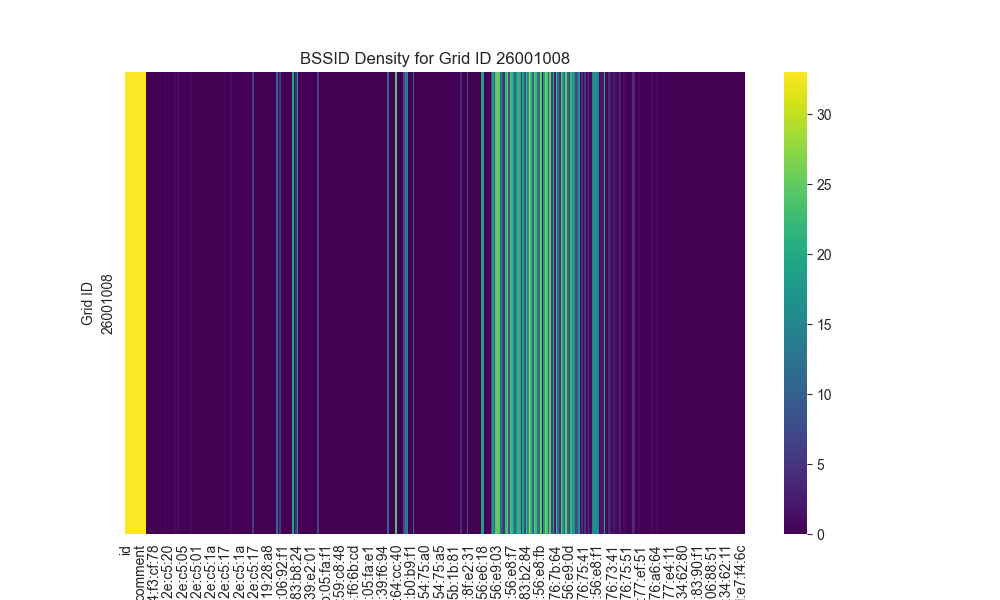
\includegraphics[width=1.25\linewidth]{heatmap_gridid_26001008.png}\par\medskip
			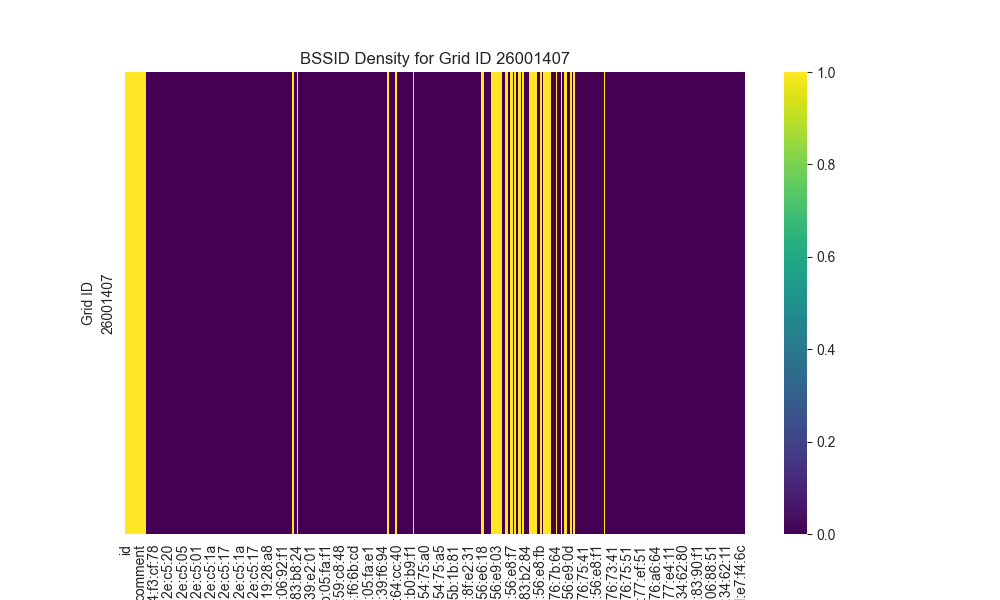
\includegraphics[width=1.25\linewidth]{heatmap_gridid_26001407.png}\par\medskip
			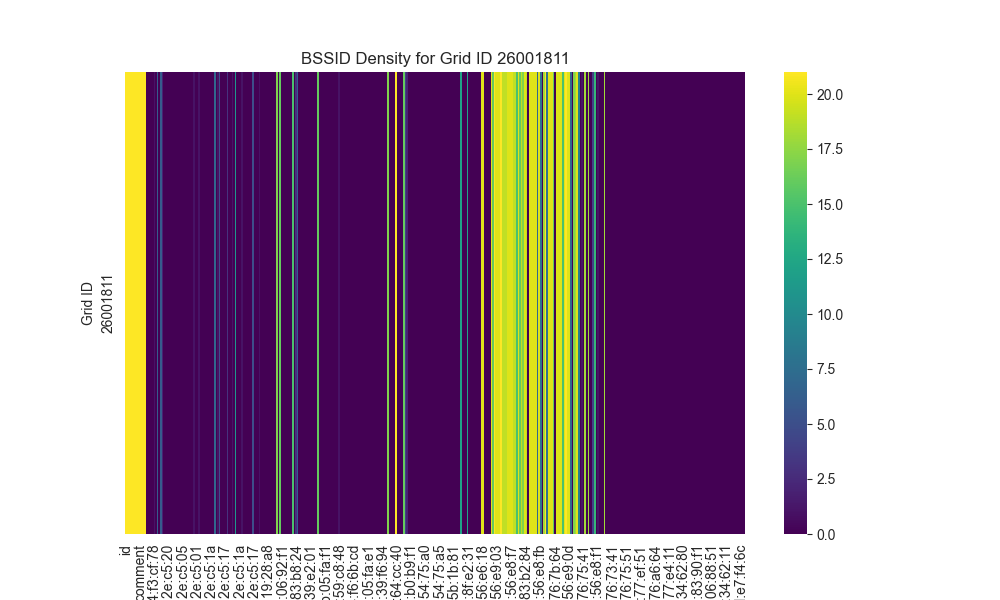
\includegraphics[width=1.25\linewidth]{heatmap_gridid_26001811.png}\par\medskip
			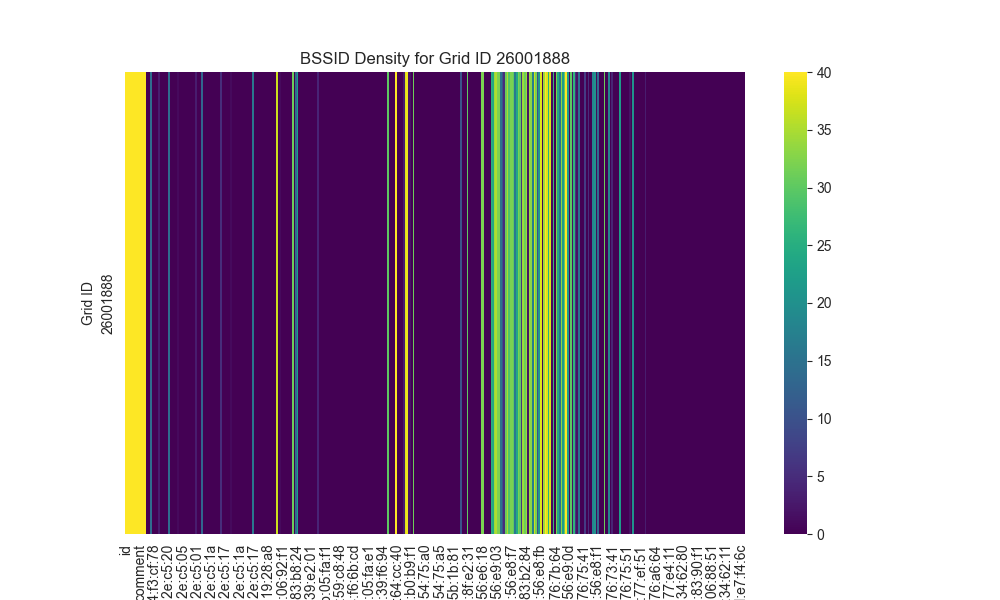
\includegraphics[width=1.25\linewidth]{heatmap_gridid_26001888.png}\par\medskip
			%\subfloat[Grid ID 260011369]{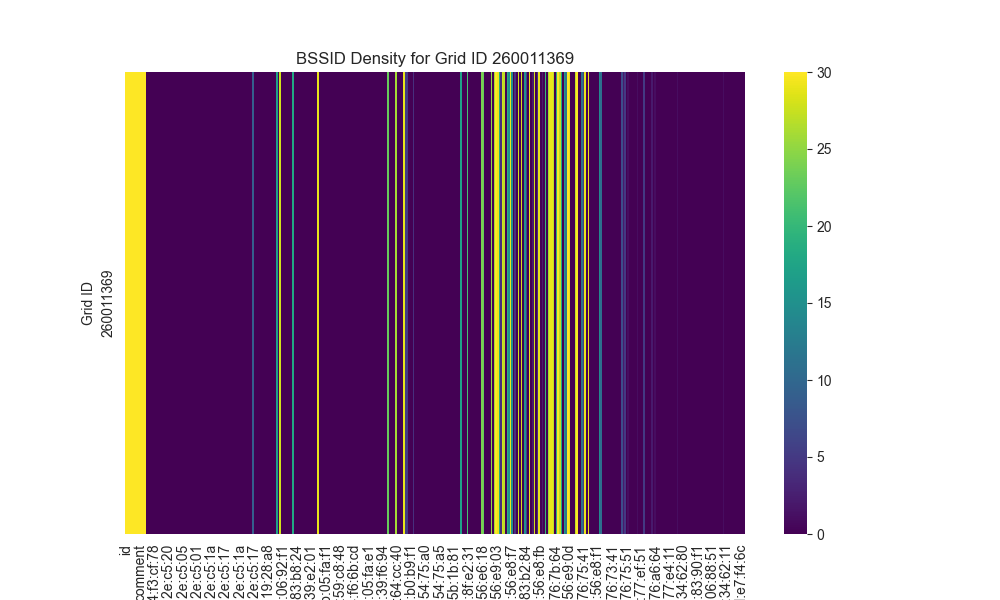
\includegraphics[width=1.25\linewidth]{heatmap_gridid_260011369.png}}
		\end{minipage}
		\hfill
		% Right Column (27XXXX IDs)
		\begin{minipage}{0.45\textwidth}
			\centering
			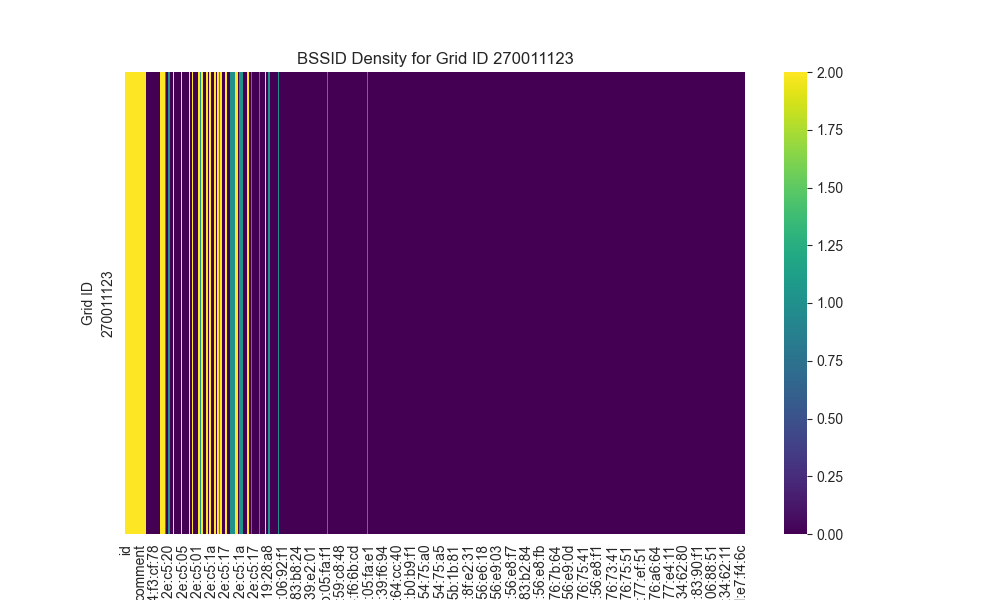
\includegraphics[width=1.25\linewidth]{heatmap_gridid_270011123.png}\par\medskip
			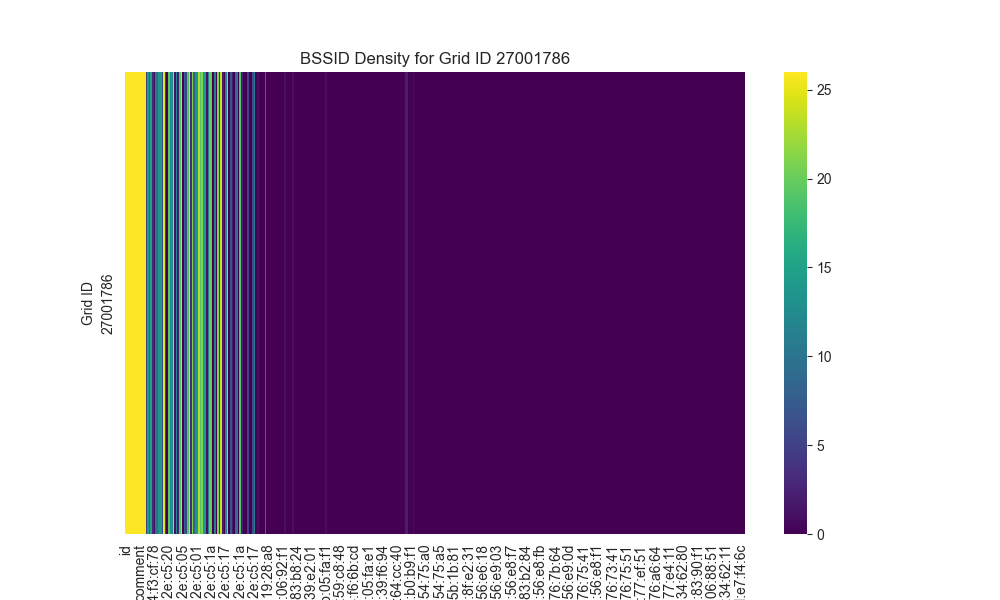
\includegraphics[width=1.25\linewidth]{heatmap_gridid_27001786.png}\par\medskip
			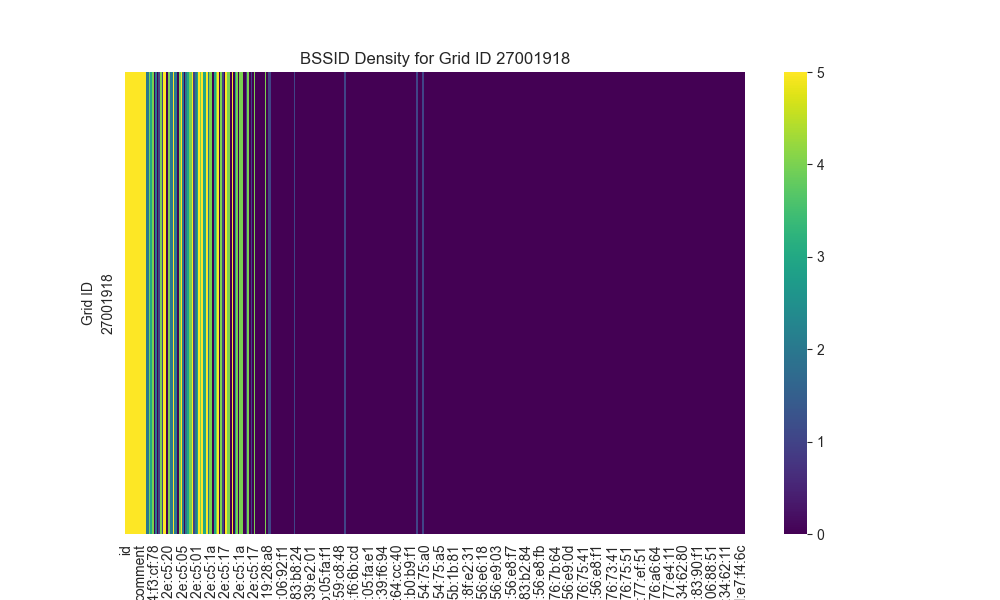
\includegraphics[width=1.25\linewidth]{heatmap_gridid_27001918.png}\par\medskip
			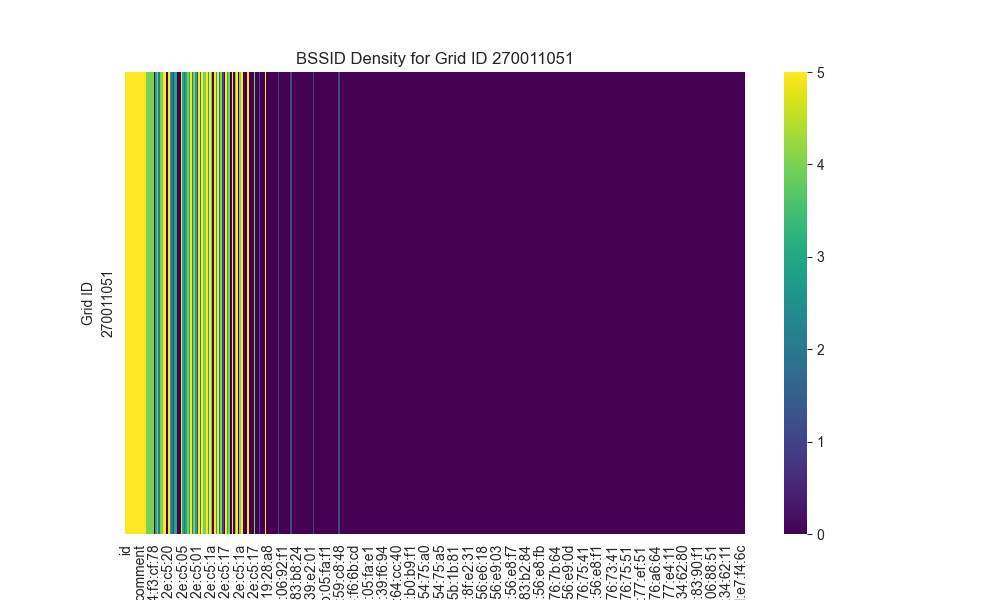
\includegraphics[width=1.25\linewidth]{heatmap_gridid_270011051.png}\par\medskip
			%\subfloat[Grid ID 270011105]{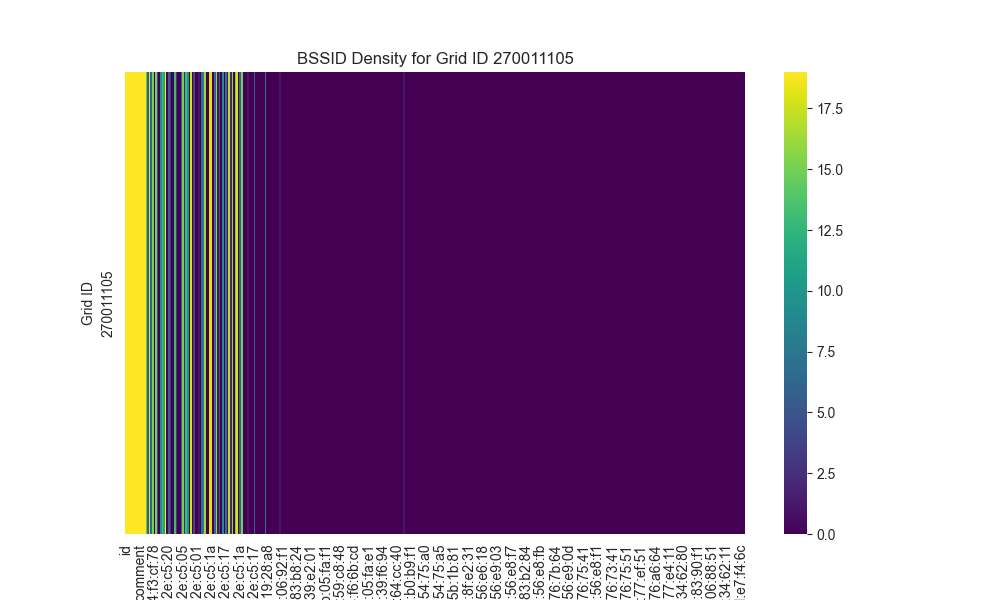
\includegraphics[width=1.25\linewidth]{heatmap_gridid_270011105.png}}
		\end{minipage}
		
		\caption{BSSID Heatmaps}
		\label{fig:bssid_heatmaps}
	\end{figure*}
	\end{comment}
\end{document}
